\documentclass[a4paper,12pt,oneside]{book}

% TODO metadata for mendeley
% TODO check spelling (ispell filename.tex)
% TODO find duplicates in labels
% TODO remove draft watermark
\usepackage{draftwatermark}
% Use the following to make modification
%\SetWatermarkAngle{45}
\SetWatermarkLightness{0.9}
%\SetWatermarkFontSize{4cm}
\SetWatermarkScale{1}
%\SetWatermarkText{DRAFT}

\usepackage[latin1]{inputenc}
%\usepackage[vcentering,right=40mm,top=20mm,left=40mm]{geometry}
%\usepackage[a4paper]{geometry}
%\usepackage[font=footnotesize, center]{caption}
\usepackage{tikz}
%\usepackage{fancyhdr}
\usepackage{verbatim}
\usepackage{listings}
\usepackage{pstricks}
\usepackage{graphics}
\usepackage{graphicx}
\usepackage{nomencl}
%\usepackage{pslatex}
\usepackage{listings}
\usepackage{listings}
\usepackage{color}
\usepackage{textcomp}
\usepackage{makeidx}
\usepackage{hyperref}
\usepackage{tocloft}
%\renewcommand{\baselinestretch}{1.5}
%\setlength{\headheight}{15pt}
\usetikzlibrary{arrows,trees}
\DeclareGraphicsExtensions{.jpg,.png}
%\renewcommand{\chaptername}{}
%\renewcommand{\thechapter}{}
\lstset{
        language=[Visual]C++,
        keywordstyle=\bfseries\ttfamily\color[rgb]{0,0,1},
        identifierstyle=\ttfamily,
        commentstyle=\color[rgb]{0.133,0.545,0.133},
        stringstyle=\ttfamily\color[rgb]{0.627,0.126,0.941},
        showstringspaces=false,
        basicstyle=\small,
        tabsize=2,
        breaklines=true,
        prebreak = \raisebox{0ex}[0ex][0ex]{\ensuremath{\hookleftarrow}},
        breakatwhitespace=false,
        aboveskip={1.5\baselineskip},
  columns=fixed,
  upquote=true,
  extendedchars=true,
 frame=single,
 escapeinside={(*@}{@*)},
}
\hypersetup{
	pdftitle={Grid Monitoring},
	pdfauthor={Theofylaktos Papapanagiotou},
	pdfsubject={Grid Computing},
	baseurl={http://people.brunel.ac.uk/~dc09ttp/grid_monitoring.pdf},
	pdfdisplaydoctitle={true},
	pdffitwindow={false},
	pdfkeywords={grid monitoring, ganglia},
	pdfprintscaling={None},
	pdfpagelayout={TwoPageLeft},
	setpagesize={true},
}
% There is no restriction on font. Times Roman is acceptable; size must be around 12 point.
\usepackage[T1]{fontenc}
\usepackage{times}
% The text should be double-spaced, with a 40 mm margin on the left-hand side of the pages and 20 mm top and bottom margins.
\usepackage{setspace}
\doublespacing
\pagestyle{headings}
%\setlength{\hoffset}{-1in}
%\setlength{\voffset}{-1in}
%\addtolength{\textheight}{20mm}
\addtolength{\hoffset}{-1in}
\addtolength{\hoffset}{20mm}
\addtolength{\voffset}{10mm}
\addtolength{\voffset}{-1in}
\oddsidemargin=20mm
\topmargin=5mm
\headheight=10mm
\headsep=5mm
\textheight=257mm
\textwidth=130mm
\marginparsep=20mm
\marginparwidth=20mm
\footskip=10mm
%\renewcommand{\headrulewidth}{1pt}
%\renewcommand{\footrulewidth}{1pt}
%\addtolength{\headheight}{0pt}
%\fancyfoot[L]{Grid Monitoring}
%\fancyfoot[RO]{Theofylaktos Papapanagiotou}
%\addtolength{\textheight}{70pt}
%\setlength{\marginparwidth}{40mm}
%\usepackage{layout}



\makenomenclature
\makeindex

\begin{document}
%\layout

\frontmatter

\thispagestyle{empty}

\begin{center}
\Large
School of Engineering \& Design\\
Electronic \& Computer Engineering\\
\vspace{1\baselineskip}

MSc in Data Communications Systems\\
\vspace{1\baselineskip}

\begin{center}

\includegraphics[width=40mm]{images/brunel_logo}\\
\end{center}
\vspace{0.5\baselineskip}

\Huge
Grid Monitoring\\
\vspace{1.5\baselineskip}
\Huge
Theofylaktos Papapanagiotou\\
Dr.Paul Kyberd\\
\vspace{1\baselineskip}
\large
March 2011\\
\vspace{0.5\baselineskip}
\large
A Dissertation submitted in partial fulfillment of the\\
requirements for the degree of Master of Science
\end{center}
\thispagestyle{empty}

\begin{center}
\Large
School of Engineering \& Design\\
Electronic \& Computer Engineering\\
\vspace{1\baselineskip}

MSc in Data Communications Systems\\
\vspace{1\baselineskip}

\begin{center}
\includegraphics{images/brunellogo.jpg}\\
\end{center}
\vspace{1\baselineskip}

\Huge
Grid Monitoring\\
\vspace{2\baselineskip}
\Large
Student's name: Theofylaktos Papapanagiotou \\
Signature of student: \\

\vspace{1.8\baselineskip}
\large
{\bf Declaration}: I have read and I understand the MSc dissertation\\
guidelines on plagiarism and cheating, and I certify that this\\
submission fully complies with these guidelines.
\end{center}
\section*{Abstract}
%description: Develop an interface which allows the customisable aggregation and display and information on the performance of a computational grid.

EGI has been replaced EGEE in as the main European Grid Initiative. Multi Level Monitoring architecture suggested central points in regional level where metrics from each information system of the grid will be aggregated. MyEGI, MyEGEE and Nagios replace SAM in availability monitoring. Performance monitoring is approached using Ganglia as the source of performance metrics, and WSRF/BDII as the carier of that information.

Both Globus and gLite resource brokers come with their favorite information service. Grid Monitoring Architecture suggests the model by which the information should be discovered and transfered. Monitoring and Discovery Service is responsible to provide that information. Two different methods exist about the way that the information is transfered, BDII and WSRF. Both are implementing the Glue schema, support Information Providers, and export the metrics in standard formats.

Linux kernel load average is the main metric that is taken by Ganglia, and through the information providers is passed to Nagios, LDAP and the container that supports the WSRF. Ganglia distribute the metrics to all its nodes using XDR over the multicast network. Nagios store the historical data using NDOUtils to its database repository. Ganglia python client is integrated with BDII LDAP to provide real-time metrics of Gmond to information consumers. WSRF transforms through XSLT the XML taken by Gmond and passes it to the framework's Index to be discovered and aggragated.

Finally, data are represented in graphs using RRDtool through pnp4nagios plugin of Nagios system. LDAP queries using PHP provide the real-time data from BDII. DOM library of PHP used to parse data using XPath queries in WebMDS frontend of WSRF.

\clearpage

%TODO level 3 for debugging, turn back to 1
\setcounter{tocdepth}{3}
\tableofcontents
%\printnomenclature
%\clearpage

%Initiatives
\nomenclature{EGEE}{Enabling Grids for E-sciencE Project}
\nomenclature{EGI}{European Grid Infrastructure}
\nomenclature{NGI}{National Grid Initiative}
\nomenclature{ROC}{}
\nomenclature{GGUS}{}
\nomenclature{LT2}{London Tier 2 of GridPP}
\nomenclature{Gridpp}{UK Computing for Particle Physics}
\nomenclature{NGS}{National Grid Service}

Academic
\nomenclature{CERN}{European Organization for Nuclear Research}
\nomenclature{CMS}{}
\nomenclature{ATLAS}{}
\nomenclature{ALICE}{}
\nomenclature{LHCb}{}
\nomenclature{WLCG}{Worldwide LHC Computing Grid}

Resource brokers
\nomenclature{Globus}{}
\nomenclature{gLite}{}
\nomenclature{WMS}{}
\nomenclature{}{}

The information system
\nomenclature{ATP}{Aggregated Topology Provider}
\nomenclature{MRS}{Metric Result Store}
\nomenclature{MDDB}{Metric Description Database}
\nomenclature{OIM}{}
\nomenclature{OSG}{}
\nomenclature{GOCDB}{Grid Operations Centre DataBase}
\nomenclature{BDII}{Berkeley Database Information Index}
\nomenclature{Glue}{}
\nomenclature{LDAP}{}
\nomenclature{LDIF}{}
\nomenclature{OGF}{Open Grid Forum}

Monitoring
\nomenclature{SAM}{}
\nomenclature{Nagios}{}
\nomenclature{NRPE}{}
\nomenclature{MDS2}{}
\nomenclature{GIIS}{}
\nomenclature{GRIS}{}
\nomenclature{GMA}{}
\nomenclature{R-GMA}{}

c-COD
CICDB
COD
DownCollector
EGI\_DS
EUMedGrid
Ganglia
Gratia
Gstat
LEMON
MonALISA
MRTG
Nagios
NCG
RAL
r-COD
RTM
SAM
SGAS
SLD
SPOF
TPM
VOCard
WiatG
WLCG
Zabbix
APEL
BDII
DGAS
EELA
ENOC
EUGridPMA
GLUE
GOC
GOCDB
GridICE
HEP
JSPG
LDAP
NGI
OSG
ROC
SLA
VOMS

\printnomenclature[3cm]
\listoftables
\lstlistoflistings
\listoffigures

\pagestyle{fancy}
\renewcommand{\headrulewidth}{1pt}
\renewcommand{\footrulewidth}{1pt}
\addtolength{\headheight}{0pt}
\fancyfoot[L]{\thepage}
\fancyfoot[RO]{Theofylaktos Papapanagiotou (0940199)}
\addtolength{\textheight}{70pt}


\mainmatter

% TODO spell checking

\chapter{Introduction}
\section{Context}

\begin{figure}[htb]
\centering
\includegraphics[width=150mm]{images/gstat-architecture.jpg}
\caption{A caption}
\label{figure:alabel}
\end{figure}

\section{Aims \& Objectives}
Different role users are going to use a portal to get information about the
performance status of the grid, to export the appropriate report for their job.
This project aims to develop these particular pieces of code to support the 
aggregation of the metrics from nagios, to allow the web based customization of
the visualization of the reports. These metrics are needed to report the
availability and reliability of NGIs and particular sites of the grid.

The procedures that are going to be used in order to achieve the above aims
should include at the beggining some opening and exploration of the environment
where the interface is going to be placed. The usage of grid computing in
the world should be well known, so a visibility of the importance and the
possible uses of the software will be recognised. The appropriate
access to the infrastructure should be gained, on different platforms and levels.
Brunel University site and GridPP/NGS VO at the beggining, as long as the UKI
ROC operations may be a good point of collaboration with researchers to reach
the bests possible requirements and data to analyse. The middleware used in
both these VOs should be examined so with the knowlege of running projects and
global usage of them may target to export better specifications. Existing
operations on the grid should also be discovered. The european initiative
milestones on the operations of the regional level should be considered as a
route, and registration to news about the upcoming research projects that
are going to use the grid should also be take place.


After that wide-opening to get the whole picture, a targeted and focused
view should follow. Existing monitoring tools must be used to check the problems
and search for requirements. The experience of SAM, Gridview, Gridmap, Gstat,
GridICE, etc should be taken in order to merge their functionality as possible
as it is. Information systems that already reside over the infrastructure, must
also be learned. Standards and specifications should be examined, on how the
message bus works and delivers the data in an hierarhical manner. A contact
with the CERN team working on MyEGEE and Indiana University's MyOSG team should
be established, to collaborate on the core of MyOSG source. Changes submission
to subversion system as long as ticket closure of the development project tool
will help to get to know the core of MyEGEE and Nagios. It is possible to create
and upstream a nagios customized web interface, to create different views of
nagios resources scheme to grid topology oriented architecture. Nagios, NRPE and
Ganglia installations should be deployed across the CE\&SE nodes of Brunel's
sites to have a working production environment to work on. Attention should be
taken on the potential performance impact of these sensors deployment. UKI
MyEGEE validation/testing portal will be used as a pre-production environment
to check changes. PNP should be fixed in GridPP Nagios to be evaluated.
Statistical access log analysis of existing tools may have results on trends of
users/admins prefered views.

Various tools are going to be used to track changes and collaborate. Monitoring
articles in GridPP wiki \& CERN twiki should be made. Snippets upstream \&
status changes must be a regular operation in SVN/JIRA/Trac in CERN interfaces.
Ongoing task through the disseration project is the reading of papers and
methodical updates of Mendeley citation management tool to have the bibliography
organized. Possible changes suggestions to MSc on DCS cource notes about grid
monitoring may by made, as long as the EGI roadmap updates. Finally with the
appropriate supervision and follow-up of meetings and presentations, a paper publishing
might take place.

\section{Organization}.
\chapter{Literature Review}
\section{Grid Computing}
Grid computing \cite{li2005grid} is the most recent decade's technology innovation in high performance computing. A large number of scientists working on the operations of this huge co-operative project of EU. Monitoring \& information architecture \cite{fisher2002datagrid} has been standardized in the initial state of that project, to succeed in today scale of 150.000 cores in production. Use of grid computing nowadays takes place in academic and research environments. Also, applications in industry-based needs such as promising Power Grid control \cite{Taylor2006} are emerging.

Grid computing may be the infrastructure over which Cloud Computing may reside. Cloud computing promise that it will change how services are developed, deployed and managed. The elastic demands of education and research community is a good place where cloud computing may be developed. Many datacenters all over Europe which are currently serving grid computing infrastructure for LHC, could later share the resources to help some other big academic projects scale up as needed.

\section{Resource Brokers}
Resource Brokers \cite{Kertesz06ataxonomy} where developed to manage the workload on Computer elements and Resource elements. Globus is a non-service based RB, and gLite RB which is service based. A Workload Management System (WMS) exists in gLite to do the distribution and management of the Computing and Storage oriented tasks.

Based on the middleware that resource brokers rely on, they use the equivalent information system. From resource broker's point of view, the relevant information is the data store and query. There are two main categories of information systems in middlewares. The Directory-based and the Service-based. They are used for resource mapping by the brokers when they access the resource data.

\begin{figure}[h]
\begin{center}
% Set the overall layout of the tree
\tikzstyle{level 1}=[level distance=3.5cm, sibling distance=3.5cm]
\tikzstyle{level 2}=[level distance=3.5cm, sibling distance=2cm]

% Define styles for bags and leafs
\tikzstyle{bag} = [text width=4em, text centered, circle, thick]
\tikzstyle{end} = [circle, minimum width=3pt,fill, inner sep=0pt]

% The sloped option gives rotated edge labels. Personally
% I find sloped labels a bit difficult to read. Remove the sloped options
% to get horizontal labels. 
\begin{tikzpicture}[grow=right,sloped]
\node[bag] {Data Store and Query}
    child {
        node[bag] {WSRF}        
            child {
                node[end, label=right:
                    {MDS4}] {}
                edge from parent
                node[above] {}
                node[below]  {}
            }
            child {
                node[end, label=right:
                    {MDS3}] {}
                edge from parent
                node[above] {}
                node[below]  {}
            }
            edge from parent 
            node[above] {}
            node[below]  {}
    }
    child {
        node[bag] {LDAP}        
        child {
                node[end, label=right:
                    {MDS2}] {}
                edge from parent
                node[above] {}
                node[below]  {}
            }
            child {
                node[end, label=right:
                    {BDII}] {}
                edge from parent
                node[above] {}
                node[below]  {}
            }
        edge from parent         
            node[above] {}
            node[below]  {}
    };
\end{tikzpicture}

\caption{Grid Resource Brokers grouped by Information Systems\cite{Kertesz06ataxonomy}}
\end{center}
\end{figure}

\subsection{Globus}

Globus Toolkit is an open source toolkit used to build grids. It provides standards such as OGSA, OGSI, WSRF and GSI, and the implementations of OGF protocols such as MDS and GRAM.

\nomenclature{OGF}{Open Grid Forum}
\nomenclature{OGSA}{Open Grid Services Architecture}
\nomenclature{OGSI}{Open Grid Services Infrastructure}
\nomenclature{WSRF}{Web Services Resource Framework}
\nomenclature{MDS}{Monitoring and Discovery Service}
\nomenclature{GRAM}{Grid Resource Allocation \& Management Protocol}
\nomenclature{GSI}{Grid Security Infrastructure}

\begin{figure}[htb]
\centering
 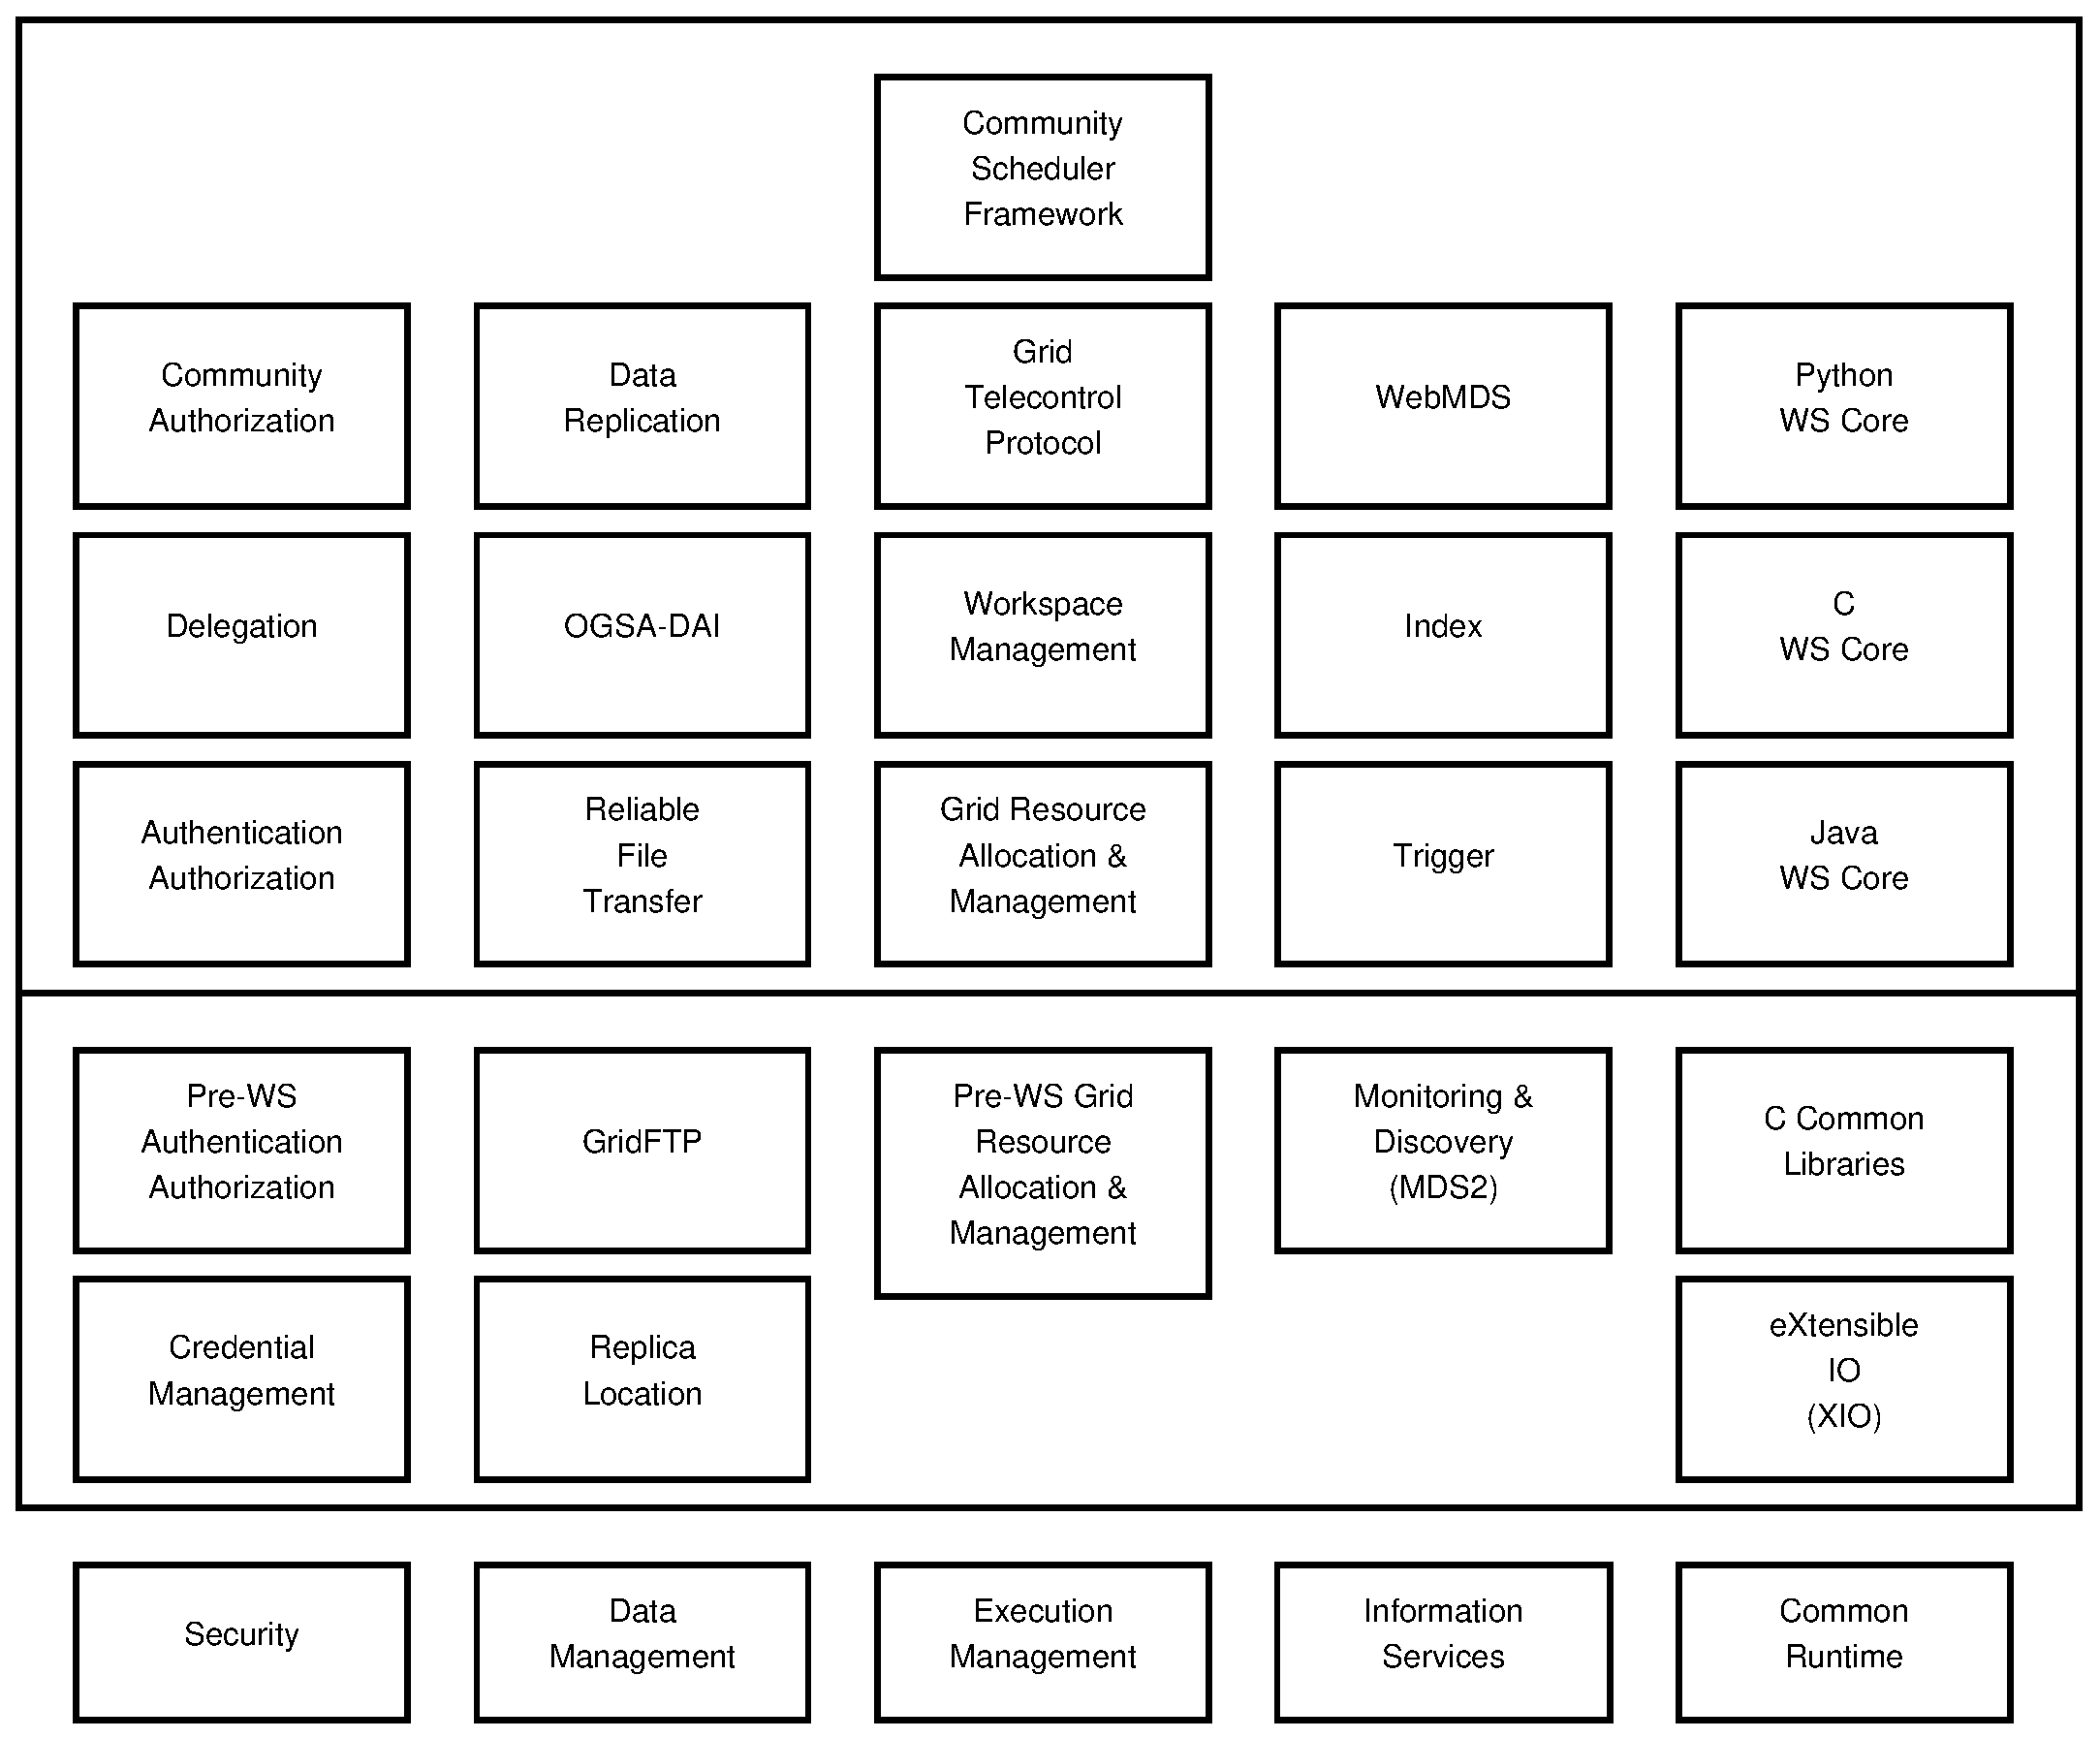
\includegraphics[width=6in]{images/globus.eps}
\caption{Globus Toolkit version 4 (GT4)}
\label{figure:globus}
\end{figure}

Monitoring and Discovery Service (MDS) is part of Globus Toolkit, and provides the information for the availability and status of grid resources. As a suite of Web Services, it offers a set of components that help to the discovery and monitoring of the resources that are available to a Virtual Organization.

\subsection{gLite}

gLite is a middleware which was created to be used in the operation of the experiment LHC in CERN. The user community is grouped in Virtual Organizations, and the security model is GSI. A grid using gLite consists of User Interface, Computer Element, Storage Element, Workload Management System and Information Service.

\begin{figure}[htb]
\centering
 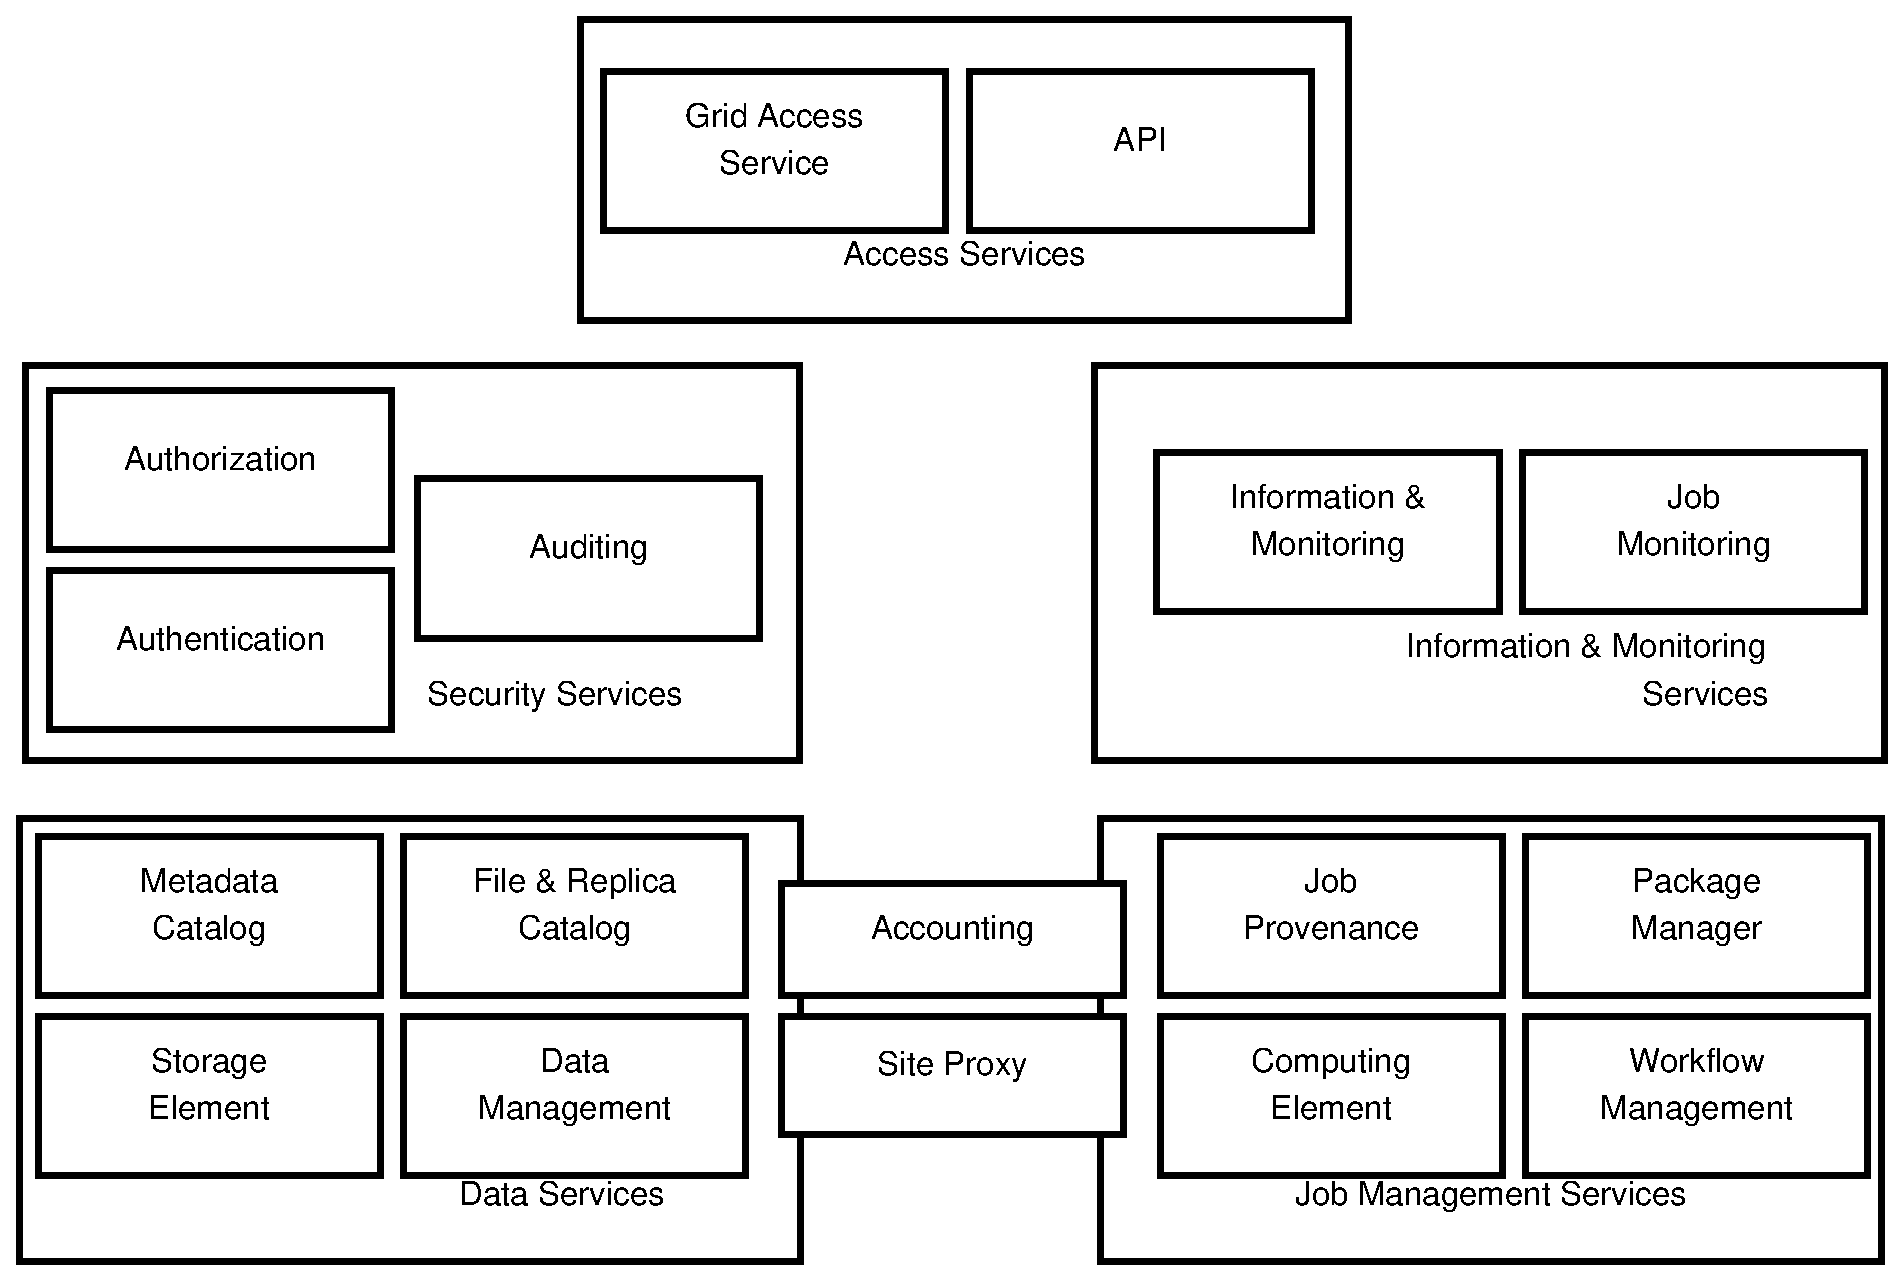
\includegraphics[width=6in]{images/glite.eps}
\caption{gLite architecture}
\label{figure:glite}
\end{figure}

The information service in version 3.1 of gLite is similar to MDS of Globus middleware, except that the GRIS and GIIS are provided by BDII (see Section \nameref{subsec:BDII}) which is an LDAP based service.

\nomenclature{BDII}{Berkeley Database Information Index}


%% TODO more about glite

\section{Information Services}
A Grid Monitoring Architecture \cite{tierney2002grid} was proposed in early 2000's. Information systems were developed to create repositories of information needed to be stored for monitoring and statistical reporting reasons. Such an organized system later was specified by the Aggregated Topology Provider (ATP) definition. The largest world grids adopt that model, forming OIM in OSG (USA) and GOCDB as that information base in EGEE (Europe). Message Bus was also defined as a mean to transfer the underlying data, and well known tools came up such as Gstat, GOCDB and BDII with Glue specification. Grid performance monitoring and keeping of such an information system has also impact in the performance of the system it shelf \cite{zhang2003performance}, so various methods were developed to give the solution to the scaling and performance problem, such as MDS2 (GIIS \& GRIS), GMA and R-GMA \cite{wilson2004information}, which offers relational environment \cite{fisher2001relational}, has experience on production systems \cite{byrom-production} and scales to reach huge needs such as CMS project \cite{Bonacorsi2004,Byrom}.

\subsection{MDS}
Monitoring and Discovery Services is about collecting, distributing, indexing and archiving information of the status of resources, services and configurations. The collected information is used to detect new services and resources, or to monitor the state of a system.

Globus Toolkit was using LDAP-based implementation for its information system since its early versions, back in 1998 \cite{von1998usage}. MDS2 in Globus Toolkit fully implemented referral with a combined GRIS and GIIS, using mds-vo-name=local to refer to the GRIS and all other strings to refer to a GIIS. It was widely accepted as a standard implementation of a grid information system \cite{945188}, with good scalability and performance \cite{zhang2004performance}.

\nomenclature{GIIS}{Grid Index Information Service}
\nomenclature{GRIS}{Grid Resource Information Service}

MDS 4 consists of the Web Services Resource Framework and a web service data browser, WebMDS. The WSRF Aggregator Framework includes:

\begin{enumerate}
  \item MDS-Index, which provides a collection of services monitoring information and an interface to query such information.
  \item MDS-Trigger, which provides a mechanism to take action on collected information.
  \item MDS-Archive, is planned for future release of MDS, to provide access to archived data of monitoring information.
\end{enumerate}

External software components that are used to collect information (such as Ganglia)\cite{gangliaWSRF} are called Information Providers.


\subsection{Glue}
As long as Information Services are used to connect different infrastructures, the schema of its structure had to be standardized. To inter-operate EU and USA grids, DataTAG developed the GLUE schema implementation. GLUE specification quickly adopted by the communities and currently its recommended LDAP DIT is specified in GLUE specification v.$2.0$ from GLUE Working Group of OSG.

Many objectclasses of the Glue schema define a Computer Element, a Storage Element, etc. As seen in Figure \ref{figure:gluece_ext} in later chapter, performance monitoring attributes such as processor load are defined in objectclasses that extends Computer Element objectclass.

\subsection{BDII}\label{subsec:BDII}
BDII is used by gLite as the Information Index Service of the LHC experiment. It is LDAP based and may be at top-level or site-level. The GIIS has been replaced by site BDII, which is fundamental for a site in order to be visible in the grid.

Top-level BDII contains aggregated information about the sites and the services they provide. Site BDII collects the information from its Computer Elements, Storage Elements, etc as long as every configured service that is installed on the site.

Information about the status of a service and its parameters is pushed on BDII using external processes. An information provider is also used (such as in WSRF) to describe the service attributes using the GLUE schema.

%% TODO make a graph about BDII
\begin{figure}[htb]
\centering
 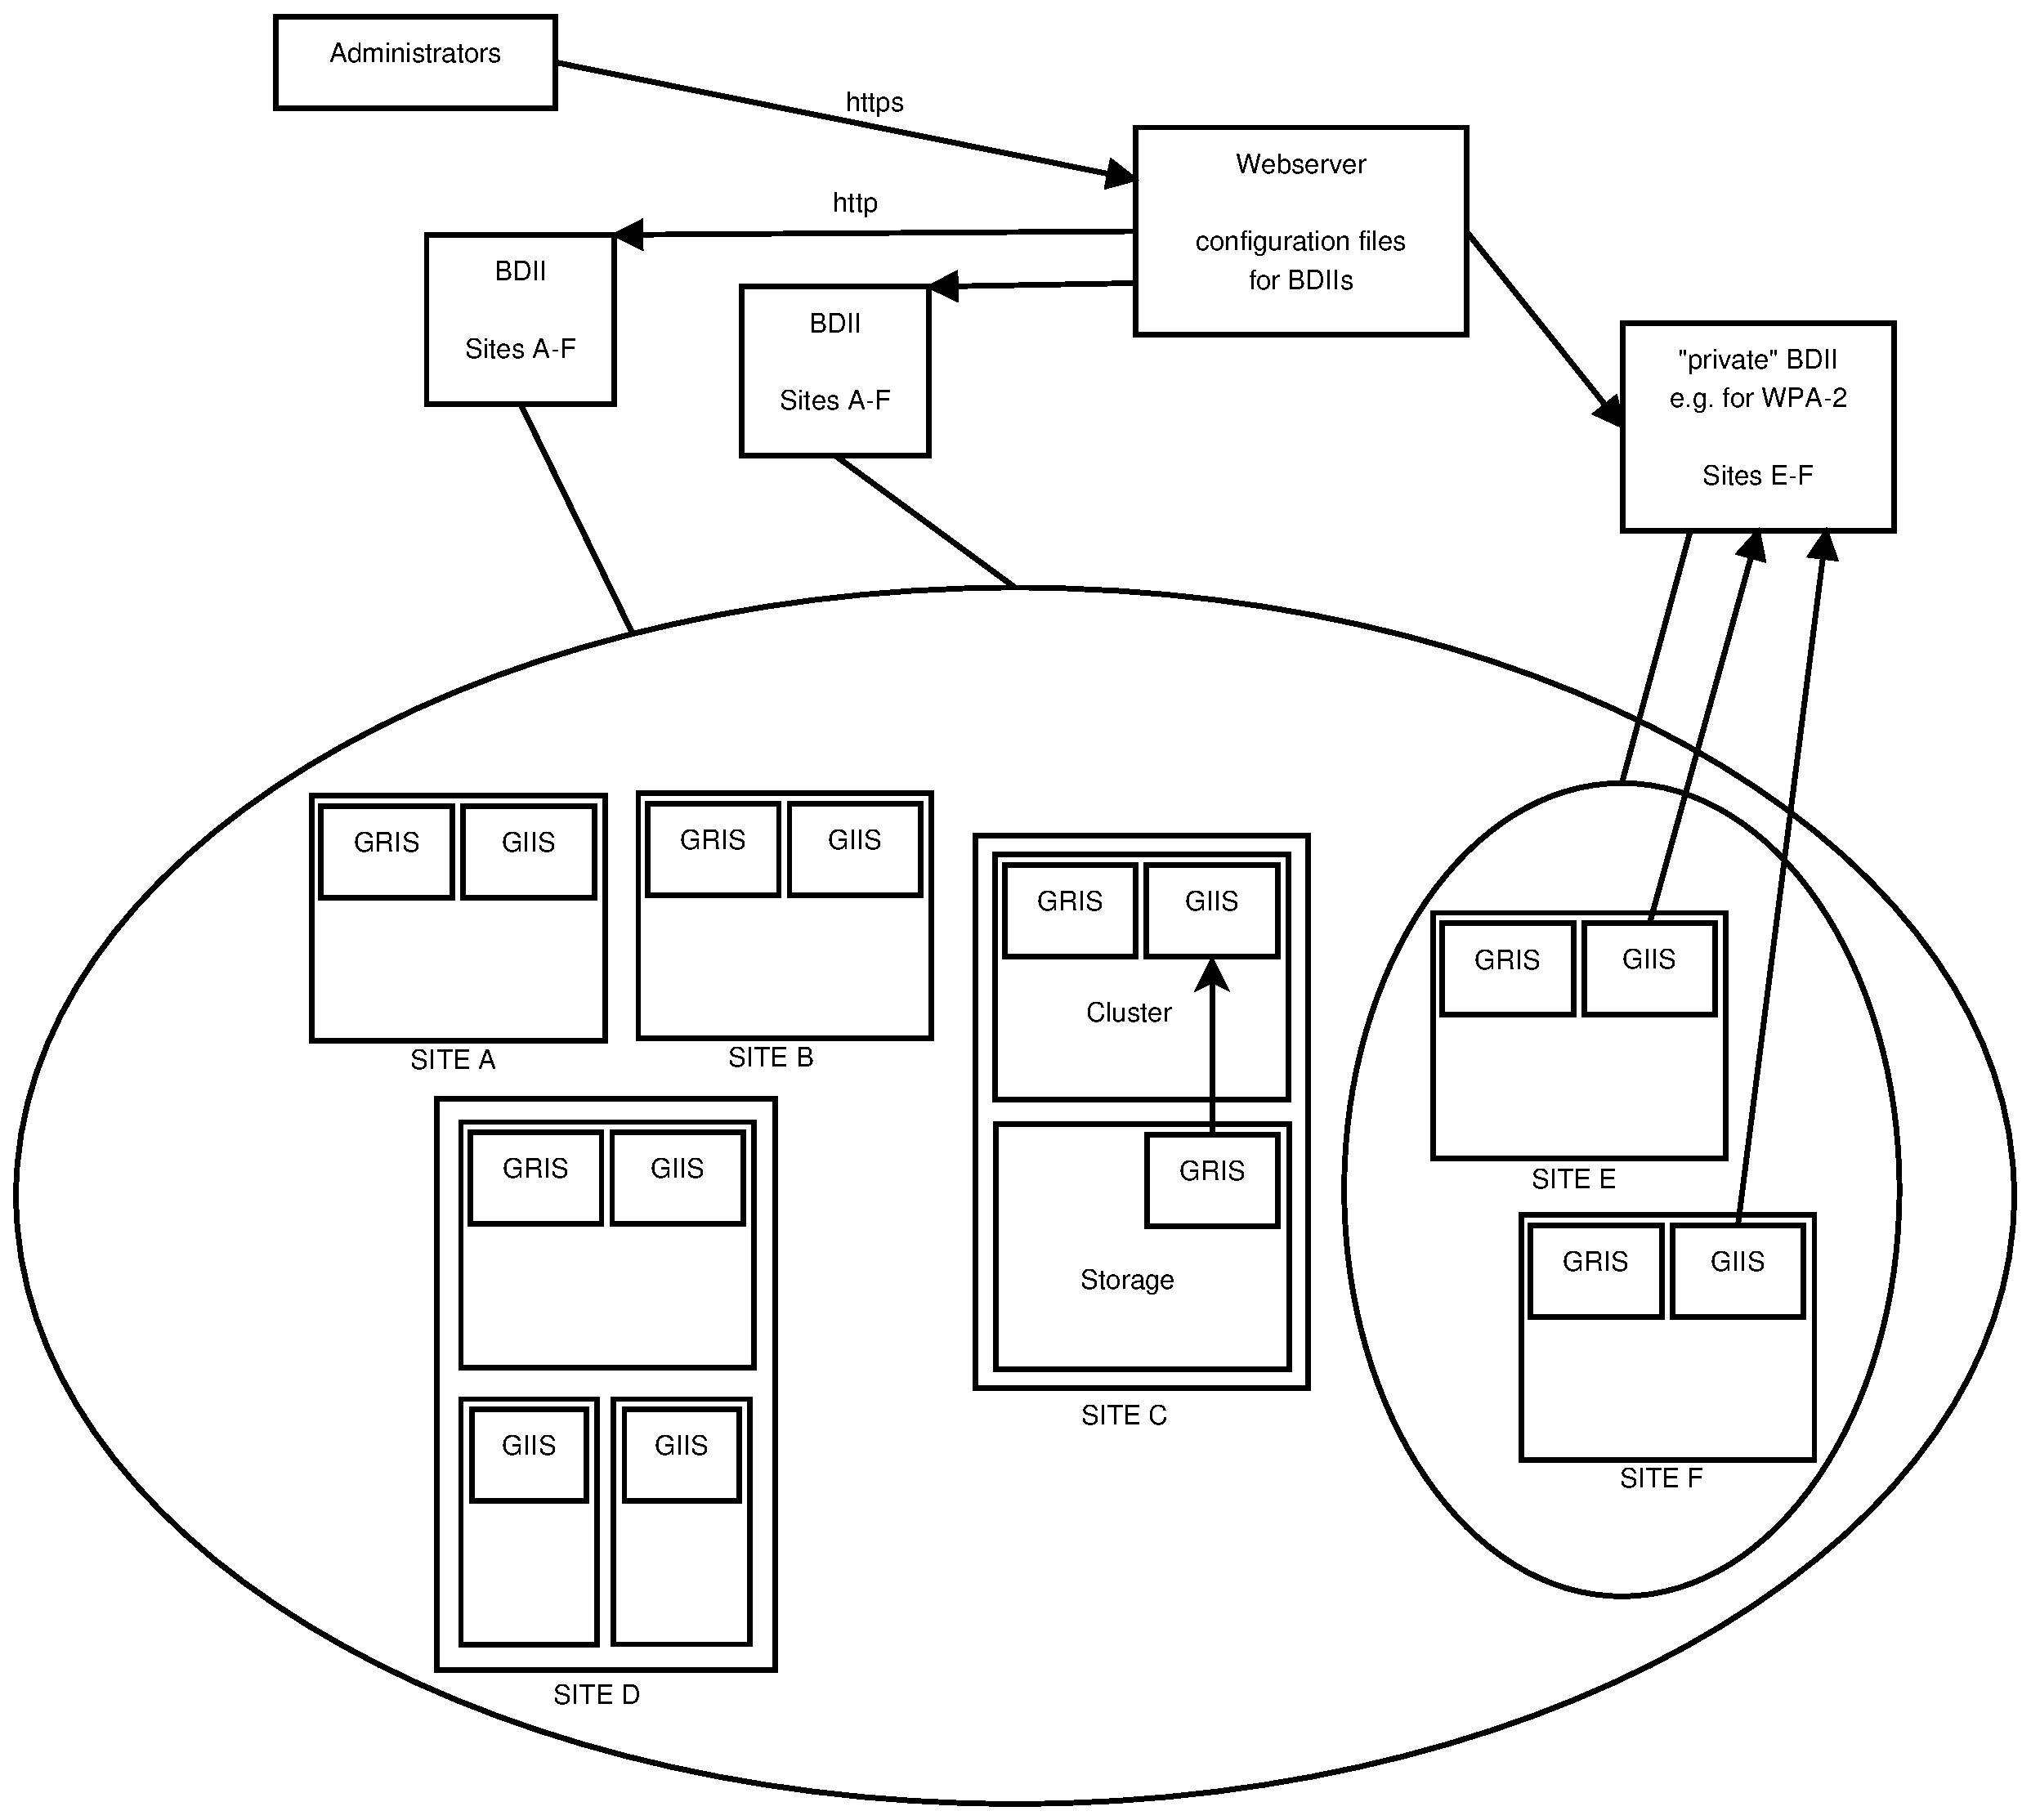
\includegraphics[width=6in]{images/bdii.eps}
\caption{Berkeley Database Information Index}
\label{figure:bdii}
\end{figure}

\section{Performance Monitoring}
%TODO those two paragraphs should be replaced or removed
Standards are being published about the operational models that the grid computing initiative will use. Last decade the EGEE I, II \& III was adopted by european universities to fund and establish a collaborative community of researchers under a central point, the CERN oriented research project in Particle Physics. After EGEE, the European Grid Initiative were formed to lead to the explode of that community into regional initiatives. Performance and availability monitoring tools and views also follow that format, phasing out commonly used SAM \cite{egee3dsa122} and having the adoption of Nagios as the monitoring of regional performance tool.


A taxonomy effort has been made \cite{gerndt2004performance} to present the differences of performance monitoring systems of the grid, and later a more general \cite{zanikolas2007importance} taxonomy paper was published to give a more general visibility of these tools. GridICE was generally used to aggregate the performance metrics of ROCs in high level reports \cite{andreozzi2005gridice}. Later GridICE was left as long as the SAM left, to meet the milestone of EGI to have a regional monitoring tool (Nagios) to report the reliability of the joined sites and report the values for SLA reasons.

Grid performance can be also measured using benchmark tools in different levels of the grid architecture, using the micro-benchmarks at the Worker Node level, the Site (CE) level and the Grid VO level. Various benchmarks exist in these levels, using different libraries and algorithms, such as This project focuses on mathematically compute of the performance of a grid based on the metrics that are taken at the Worker Node level.

Different metrics and benchmarks exist, such as the measurement of the performance of CPUs in {\bf MIPS using EPWhetstone} and the evaluation of the performance of a CPU in {\bf FLOP/s and MB/s using BlasBench}. GridBench \cite{gridbench} provides a framework to collect those metrics using its own description language, {\bf GBDL}.

GcpSensor \cite{gcpsensor} introduce a new performance metric called WMFLOPS. It uses PAPI \cite{papi} (Performance API) to access the hardware performance counters. For data distribution it uses MDS information system which provides dynamic metrics for CPU load average, one for 1, for 5 and for 15 minutes load.
%TODO add some review of linux kernel and load average

\subsection{Ganglia}

Ganglia is a monitoring tool which provides a complete real time monitoring environment. It is used by both academia and industry to monitor large installations of clusters, grids. Any number of host metrics may be monitored in real time using the monitoring core, a multithreaded daemon called Gmond. It runs on every host that is in scope of monitoring. Its four main responsibilities are:

\begin{enumerate}
\item Monitor the changes that happen in the host state
\item Multicast over the network, the changes that has been made
\item Listen to network for changes that other ganglia nodes are multicasting and
\item Answer the status of the whole cluster to specific requests, using XML.
\end{enumerate}

All the data that are gathered of the multicast channel are written to a hash table in memory. The metric data of each node that runs gmond and sends information over the multicast channel are been processed and saved. Data sent over the multicast channel is happening using external data representation (XDR). When there is a request over a TCP connection, the response is in XML.


\begin{figure}[h]
\centering
 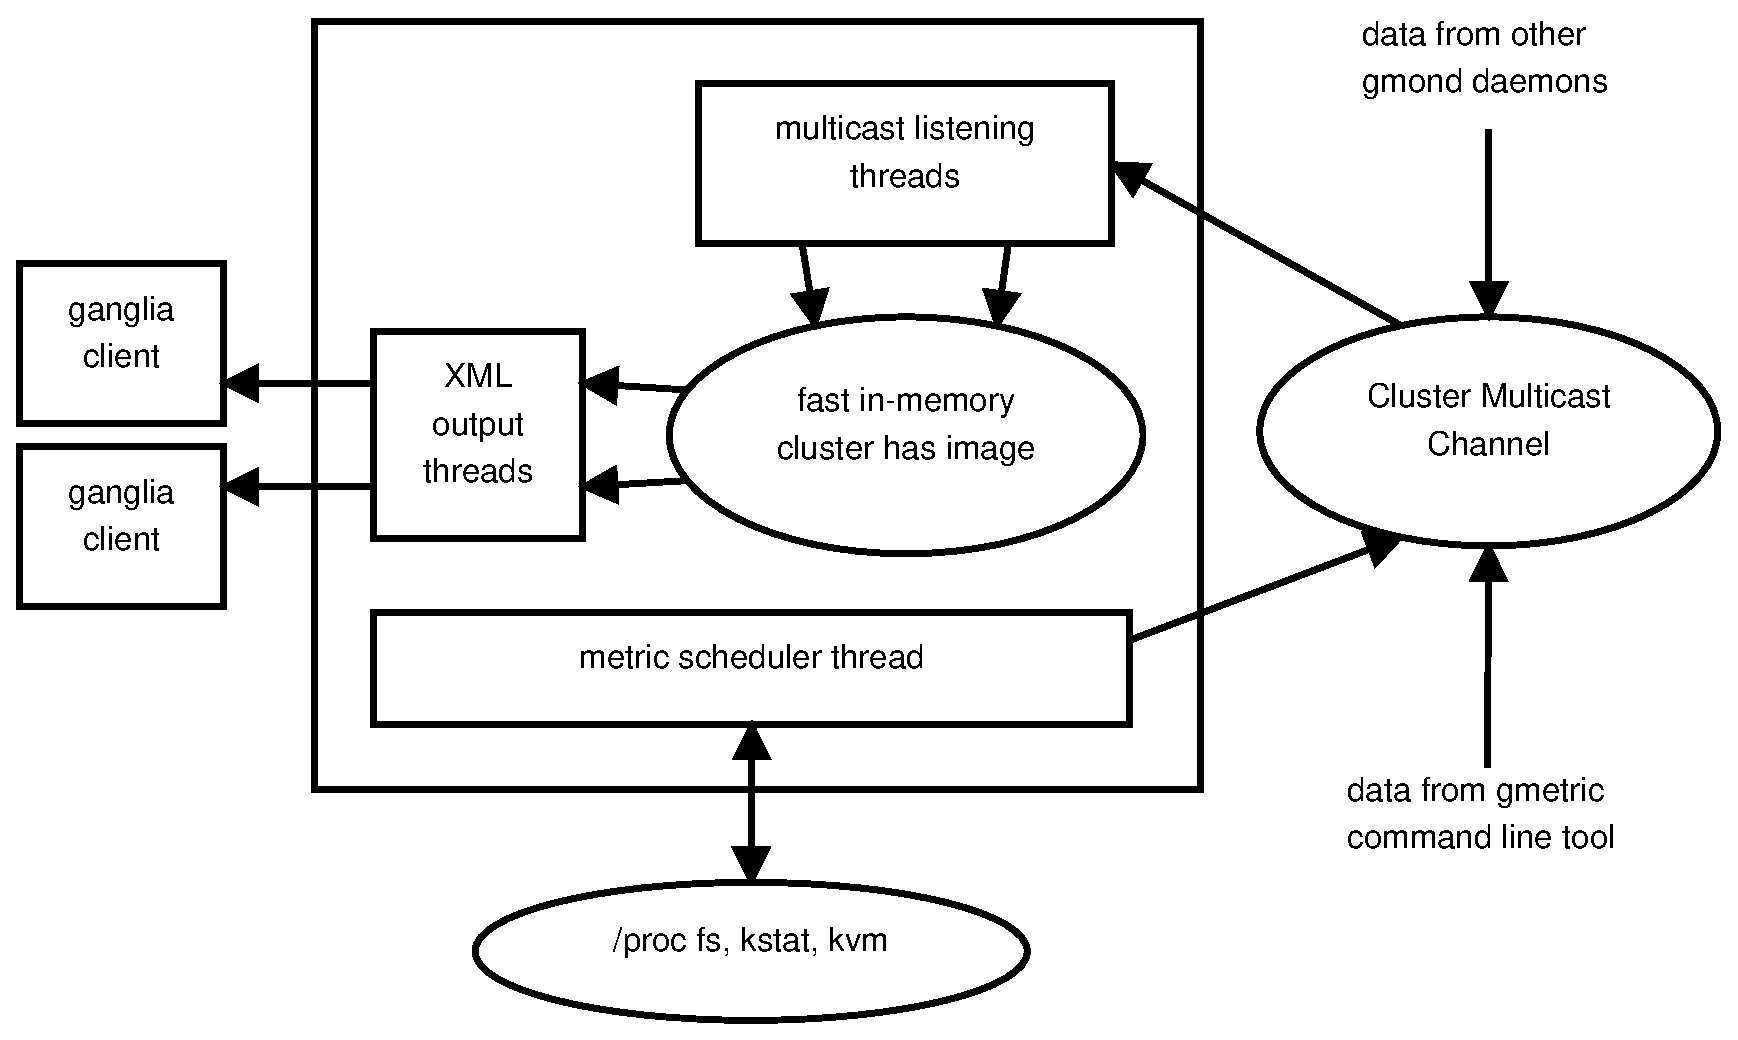
\includegraphics[width=6in]{images/ganglia.eps}
\caption{Ganglia Data Flow}
\label{figure:ganglia}
\end{figure}

\subsection{Nagios}
%TODO some literature review of nagios

\section{European Grid Infrastructure}
Latest EGI directive to form regional operation tools pushed the use of Nagios \cite{imamagic2007grid} as the main tools of availability \& performance (an so reliability) monitoring of the grid. Each NGI/ROC (regional level) has its own interface, and hierarchically there is a Super Nagios interface to report the top level view of general system availability. Nagios offers extensions such as NRPE to remotely invoke check commands in inaccessible/private installations. Another important add-on to Nagios is the NdoUtils, which offers an SQL store of history data to the monitoring interface. Nagios Configuration Generator was introduced to help the automatically generation of the configuration based on the information system of nodes and services.

Finally, there has been proposed an integration of SAM views to a Nagios customized interface, to offer the last good known SAM interface to the old users. Nagios also integrates with GGUS, a ticketing system that european grid initiative uses. Monitoring infrastructure in EGI is fully distributed using regional Nagios servers and the corresponding regional MyEGI portals.

\subsection{NGS and GridPP}
Brunel University takes part in regional and european initiatives. 5 different Computer Elements exist, and 3 Storage Elements, consisting the UKI-LT2-Brunel site. LT2 stands for London Grid, a co-operation with other London Universities. GridPP and NGS are two collaboration groups that Brunel University is member of, and papers on the web interface \cite{Hobson2007} and real time visualization of the grid status were presented \cite{Huang2007} by GridPP

In GridPP, regional monitoring tools exist to provide distributed monitoring services in UK. Regional Nagios and MyEGI/MyEGEE instances co-exist in Oxford University that offer service availability monitoring for all UK sites. Ganglia installations exist in site level deployments, and a Ganglia frontend which aggregates Tier-1 sites is offered through RAL.

\chapter{Design/Methods}
\section{Approach Adopted}

edw

to keimeno

pou tha leei

panw katw

ti ginetai

s'auto to kefalaio

DHLADH THA ESTIAZEI STO WS 'H LDAP

\newpage


\section{Design Methods}
\subsection{Recommendations and standards}
\subsubsection{Grid Monitoring Architecture}
\nomenclature{GMA}{Grid Monitoring Architecture}
%% TODO producer-consumer plot
\newpage

\subsubsection{R-GMA}
%% TODO R-GMA literature
The rgma client is no longer configured in SL5
\nomenclature{R-GMA}{Relational Grid Monitoring Architecture}


\newpage
\subsubsection{GLUE Schema}
gained wide acceptance given its adoption by Globus MDS3


GLUE schema came to provide the interoperability needed between US and European Physics Grid Projects. As a standard, a common schema was introduced to describe and monitor the grid resources. Major components include:
\begin{enumerate}
\item Computing Element (CE)
\item Storage Element (SE)
\item Network Element (NE)
\end{enumerate}

The implementation of Glue schema may be using LDAP, XML or SQL. The MDS implementation of the Glue schema in this project includes the core Information Provider and the Ganglia Interface for the cluster information.
\nomenclature{GLUE}{Grid Laboratory Uniform Environment}
\newpage

\begin{figure}[htb]
\centering
 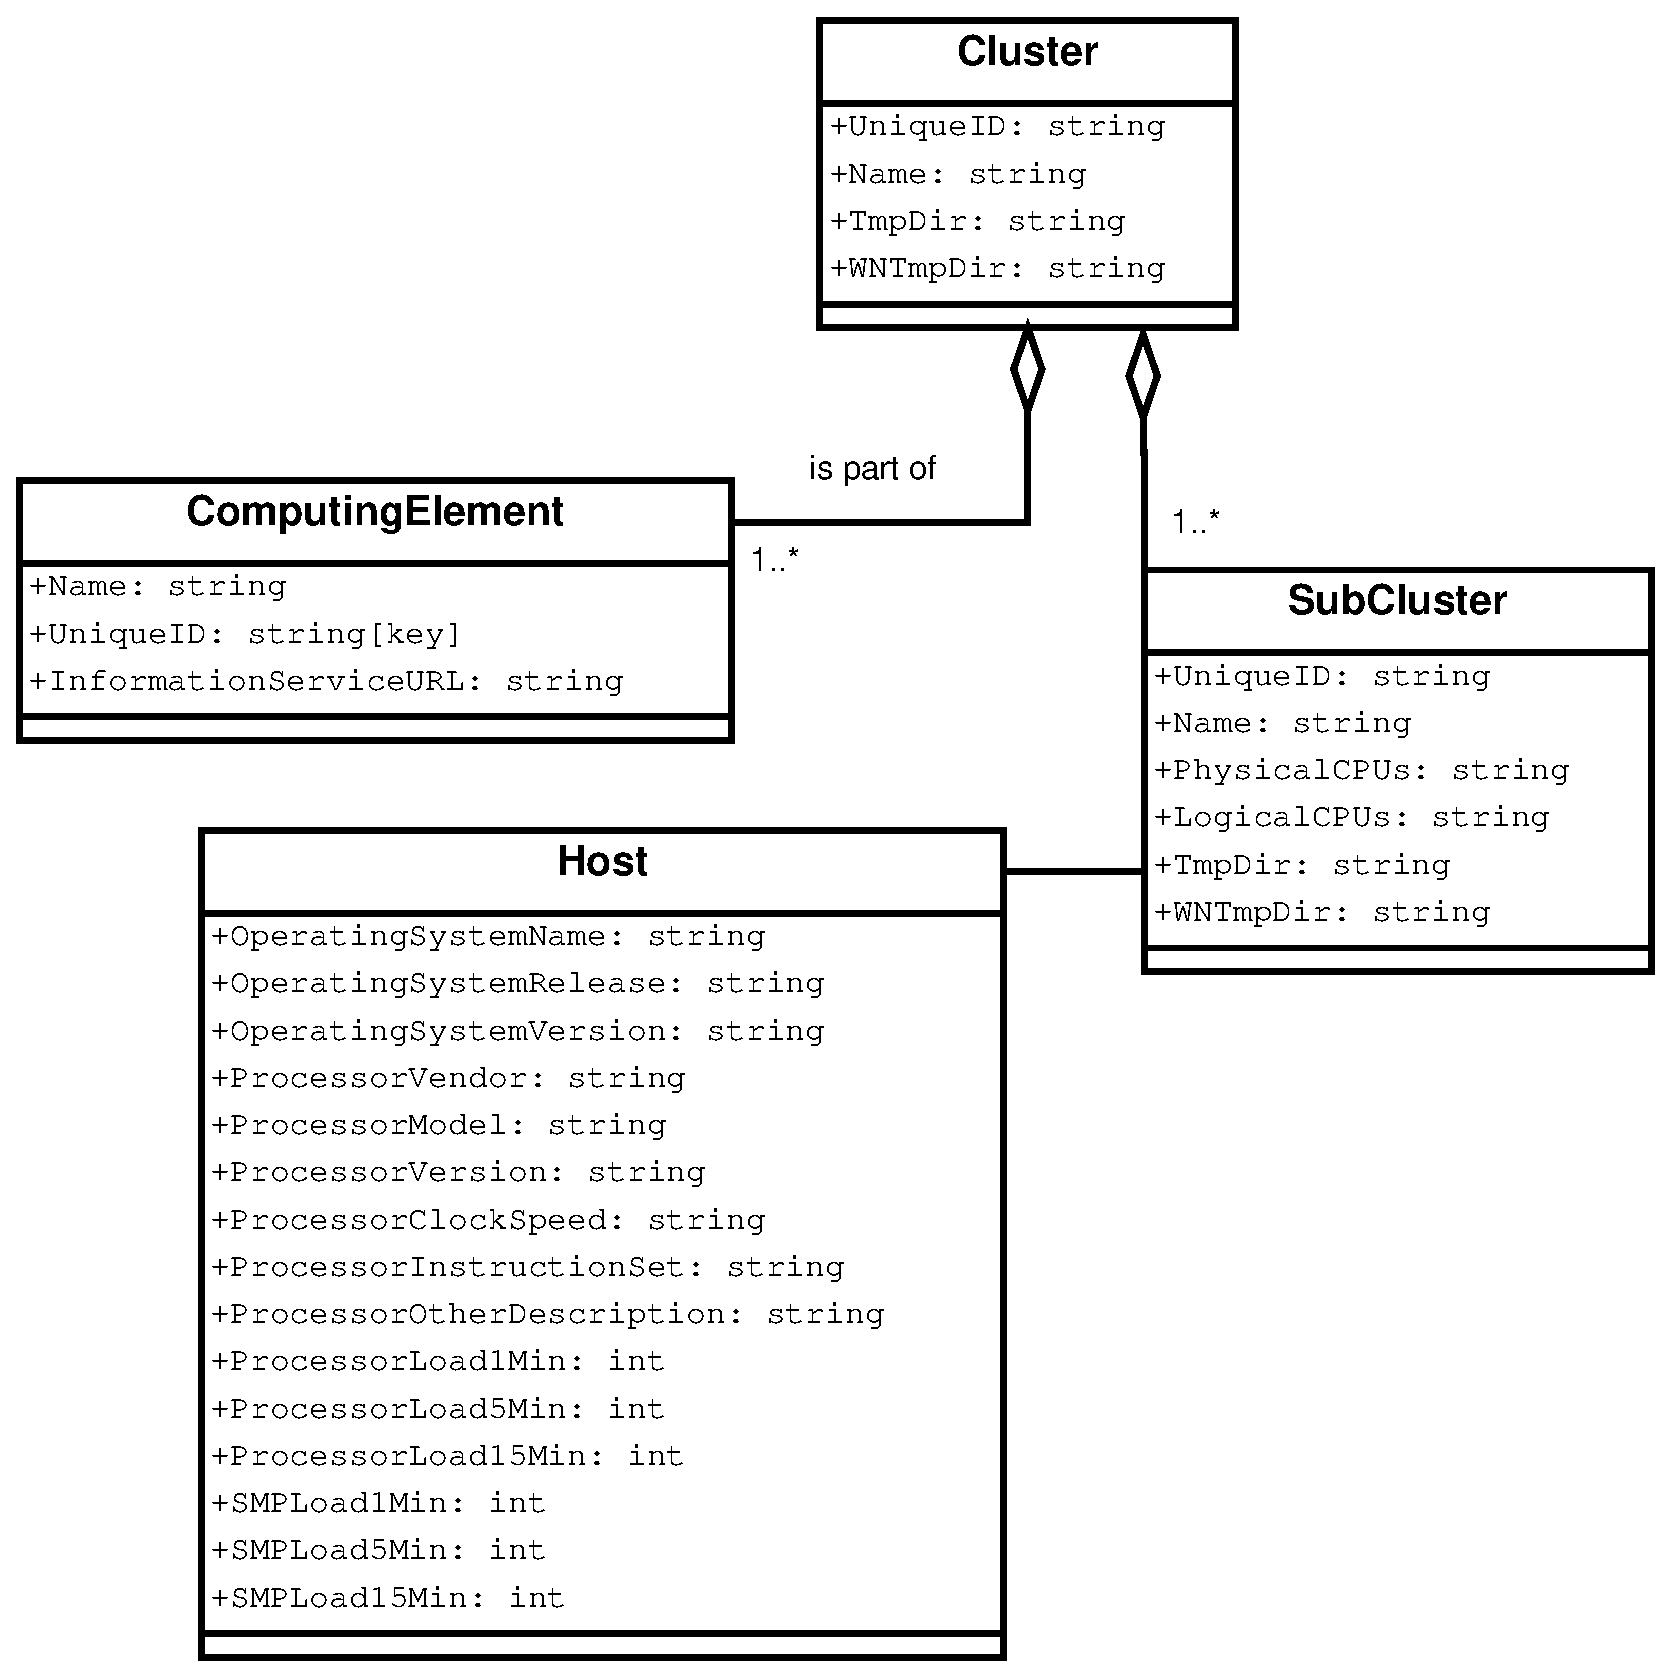
\includegraphics[width=5in]{images/gluece_ext.eps}
\caption{GLUE schema 2.0 extention for Host and SMP Load}
\label{figure:gluece_ext}
\end{figure}

\newpage

\subsection{Information Infrastructure}
% TODO to MDS me dika mou logia
``Performance''.  The applications of interest to us frequently 
operate on  a  large scale  (e.g.,  hundreds  of  proces- 
sors) and have demanding performance requirements. 
Hence, an information infrastructure must permit rapid 
access to frequently used configuration information. It 
is not acceptable to contact  a  server  for every  item: 
caching is required.
``Scalability and cost''. The infrastructure must scale to large
numbers of components and permit concurrent access
by many entities. At the same time, its organization
must permit easy discovery of information. The human
and resource costs (CPU cycles, disk space, network
bandwidth) of creating and maintaining information
must also be low, both at individual sites and in total.
``Uniformity''. Our goal is to simplify the development of
tools and applications that use data to guide configuration
decisions. We require a uniform data model
as well as an application programming interface (MI)
for common operations on the data represented via that
model. One aspect of this uniformity is a standard representation
for data about common resources, such as
processors and networks.
``The X.500 standard'' defines a directory service
that can be used to provide extensible distributed directory
services within a wide area environment. A directory service
is a service that provides read-optimized access to general
data about entities, such as people, corporations, and computers.
X.500 provides a framework that could, in principle,
be used to organize the information that is of interest to us.
\cite{mds1}
\newpage

\section{Data-acquisition Systems}
plugins that take metrics (SAM) and send results to nagios:

https://tomtools.cern.ch/confluence/display/SAMDOC/Grid+probes

http://nationalgridservice.blogspot.com/2010/10/nagios-myegee-and-myegi.html

4 layers to performance investigation:
\begin{enumerate}
  \item Storage elements
  \item Sites
  \item VOs
  \item Middleware
\end{enumerate}
3 benchmarking categories
\begin{enumerate}
  \item micro-benchmarks
  \item micro-kernels
  \item application kernels
\end{enumerate}
Benchmarking

HPL
\cite{gridbench}

CE performance
free processors
MFLOPS
MIPS (instructions per second)
free RAM

SE performance
IOPS
free space

EGI accounting portal: CPU usage metrics aggregated for accounting.
\newpage

\subsection{Metrics}

{\bf CPU load} is taken using the pseudo /proc/loadavg file which in turn is
filled by Linux kernel's CALC\_LOAD macro. This function takes 3 parameters.
The load-average bucket, a $y$ constant that is calculated using formula
\[
y=\frac{2^{11}}{2^{((5log_2(e))/60x)}}
\]
for values $x=1$, $x=5$ and $x=15$ (where x represent the minutes and y the
exponent constant), and the number of how many processes are in the queue, in
running or uninterruptible state.

\begin{figure}[htb]
\centering
 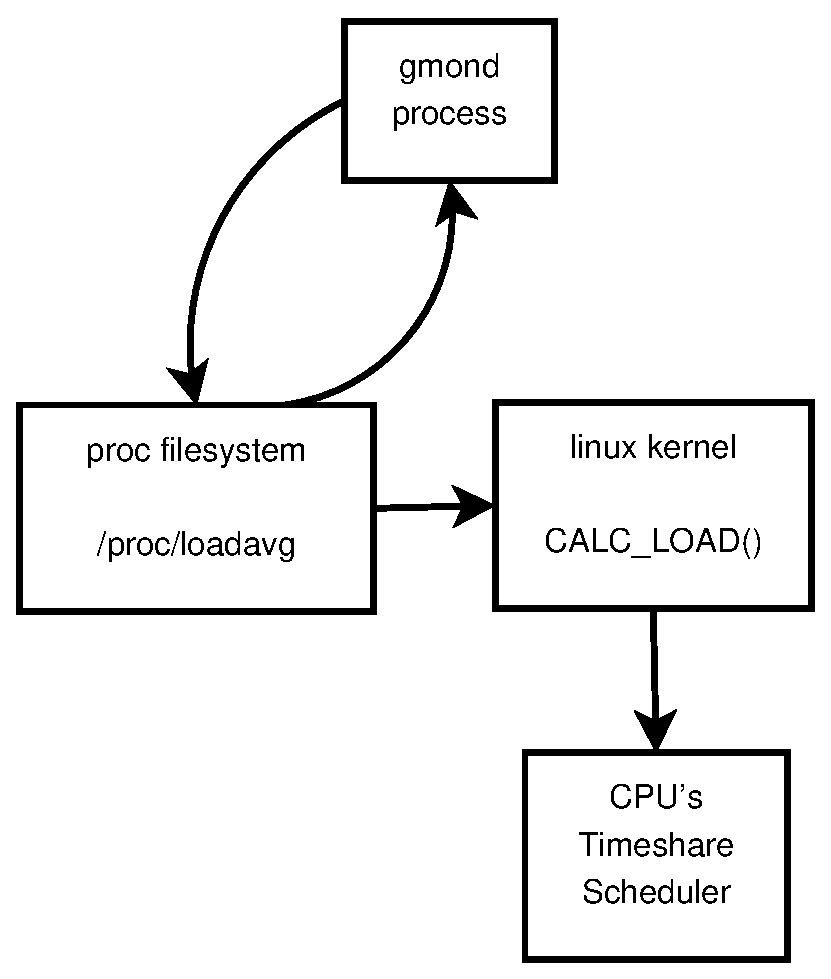
\includegraphics[width=3in]{images/calc_load.eps}
\caption{Load Average calculation}
\label{figure:calc_load}
\end{figure}

\newpage

\subsection{Ganglia}

The metrics about load in one, five and fifteen minutes are taken from Gmond daemon through the proc filesystem as seen in Figure \ref{figure:calc_load}. These values are multicasted using a UDP message on the network, only if the value has been changed from the previous one taken. There is also a time thresohold that after that time the value is been sent again, even if it haven't changed, so new hosts on the network may gather the data needed for their Gmond. Each host of a cluster have the information about the metrics of itself and each other node, so it stores the whole cluster state. Using loopback interface, every Gmond sends its metrics to itself.

If a TCP connection on the Gmond listening port 8649 is made, Gmond writes a full cluster state of metrics in XML including its DTD. There is a typical access list in the configuration called trusted hosts, and of course every node that is in the cluster that a specific node is configured to be part of, is allowed to connect to get the XML.

\begin{figure}[htb]
\centering
 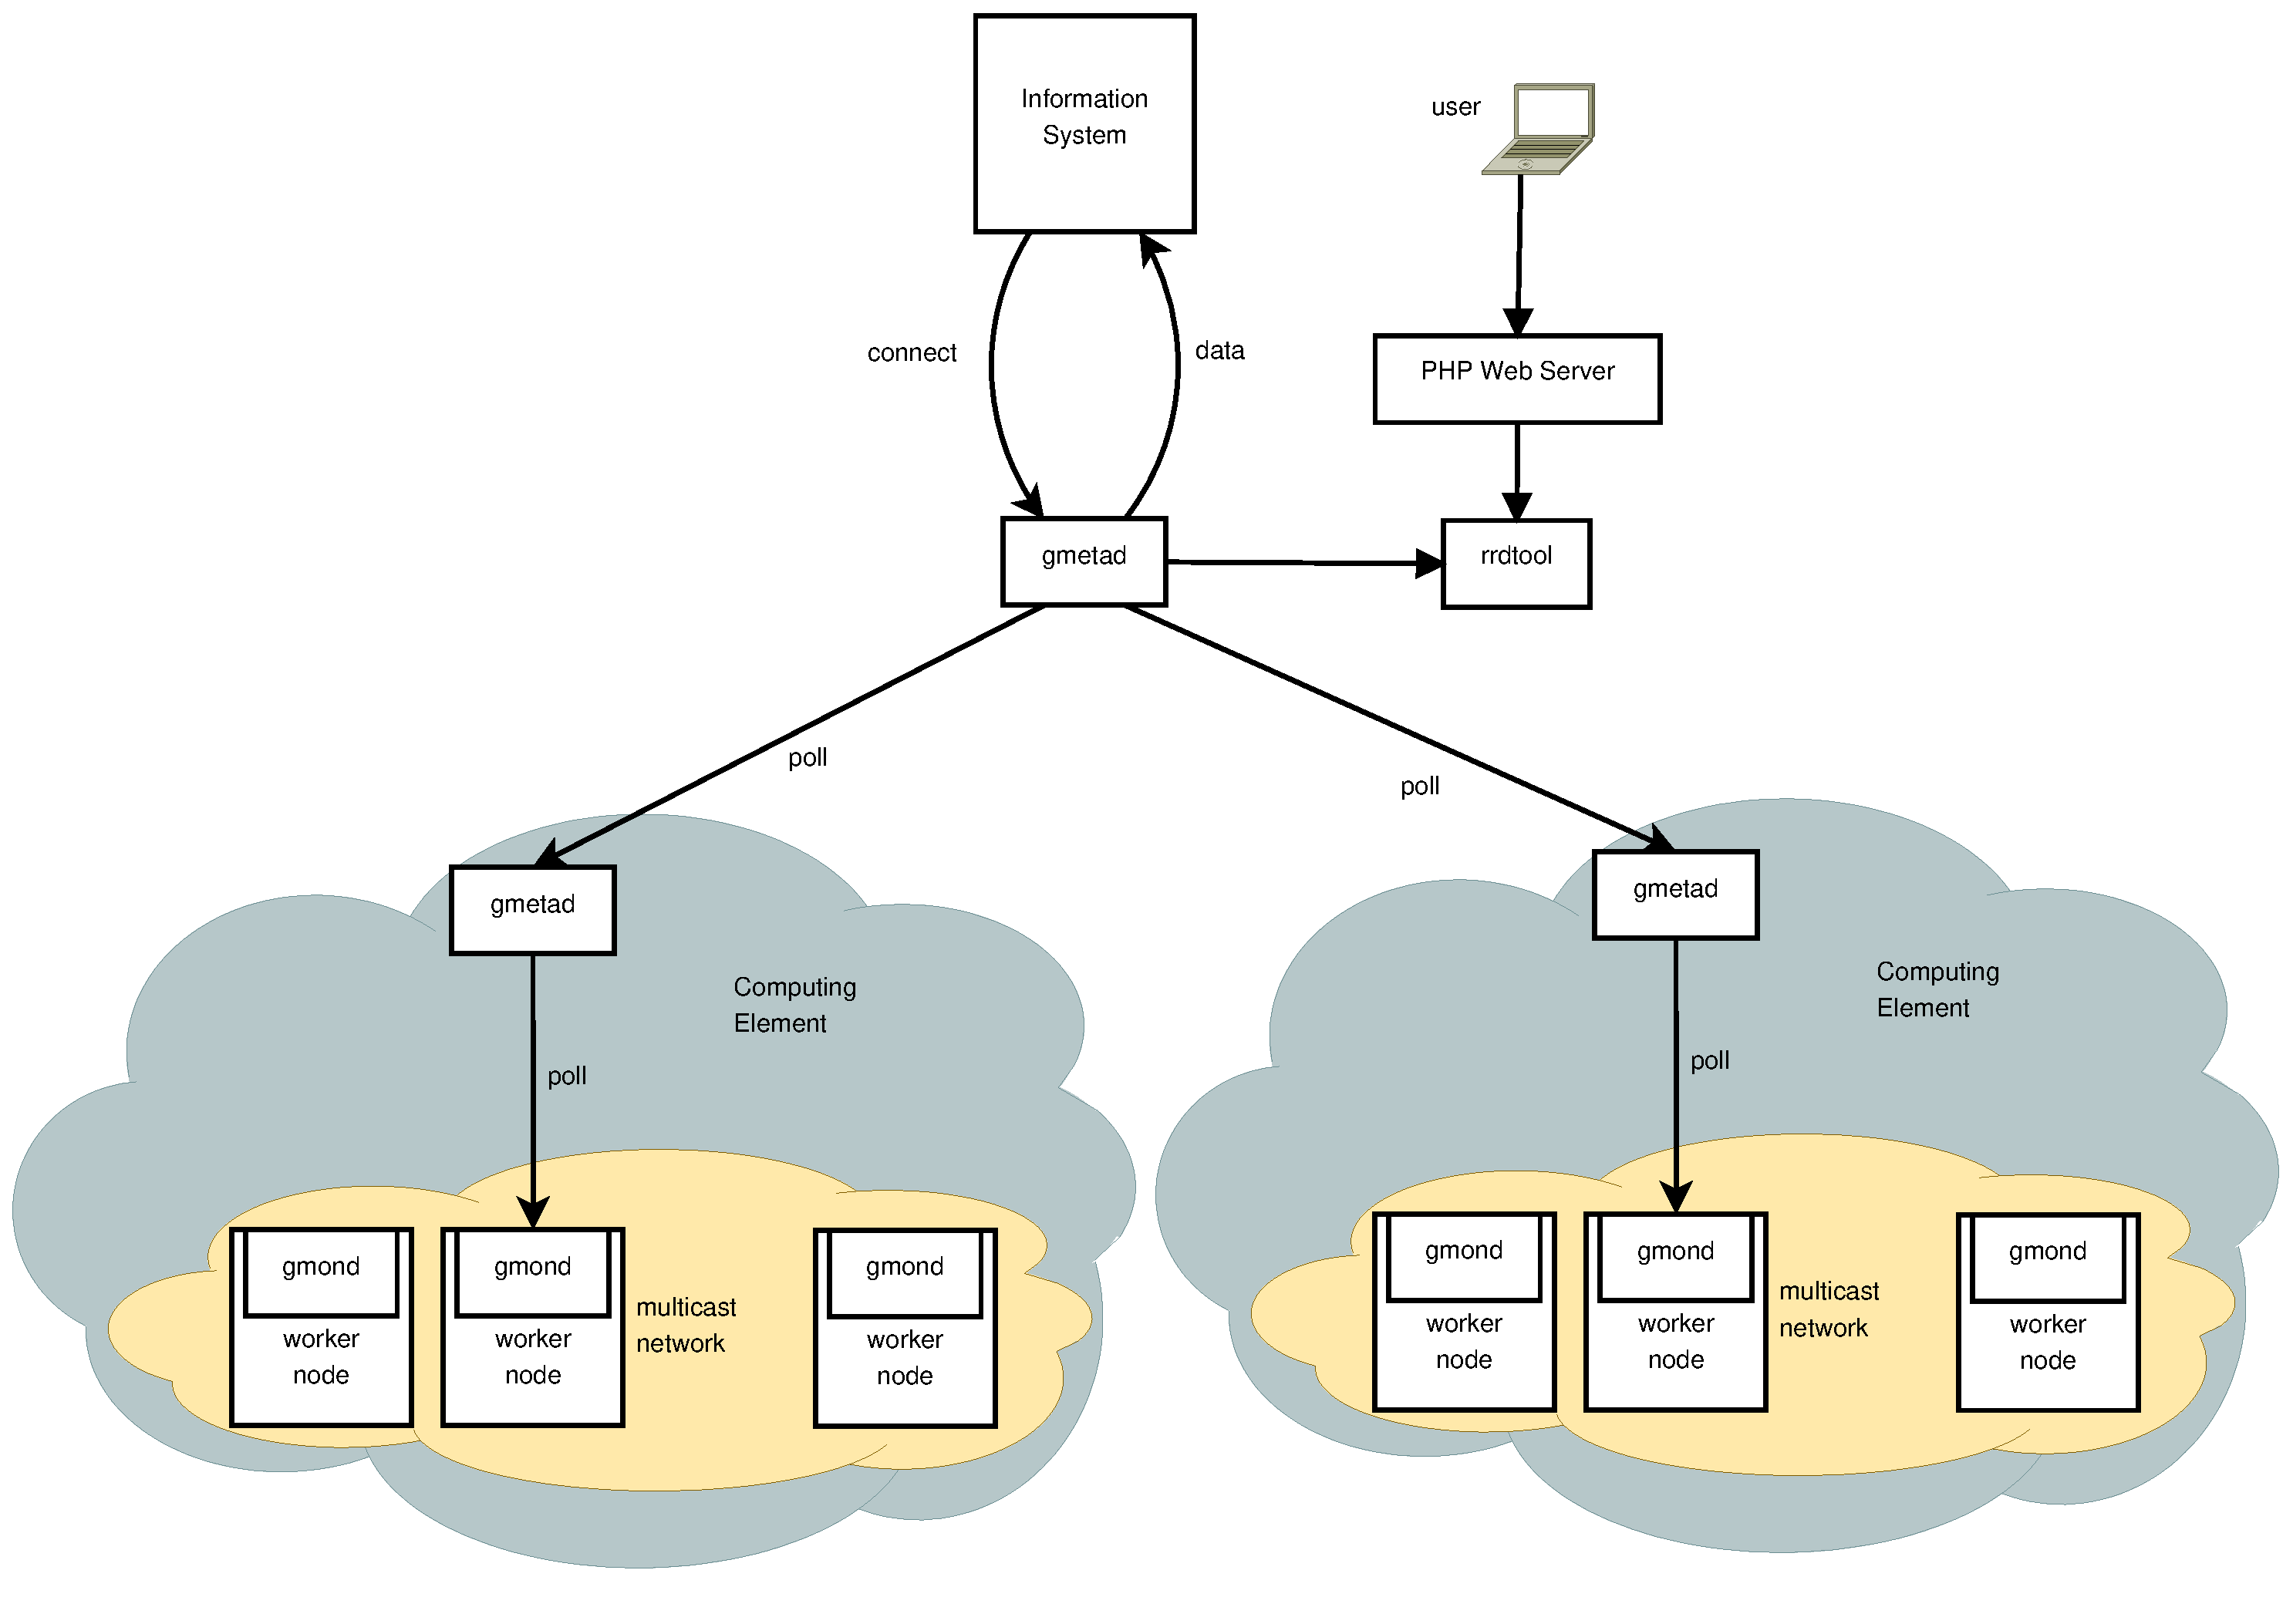
\includegraphics[width=6in]{images/ganglia_data_flow.eps}
\caption{Ganglia Network Communications}
\label{figure:ganglia_network}
\end{figure}
\newpage

\subsection{Nagios}
msg-to-handler msg-nagios-bridge
\newpage

nagios2metric
\newpage

\subsection{Ganglia to Nagios}
check\_ganglia
\begin{figure}[htb]
\centering
 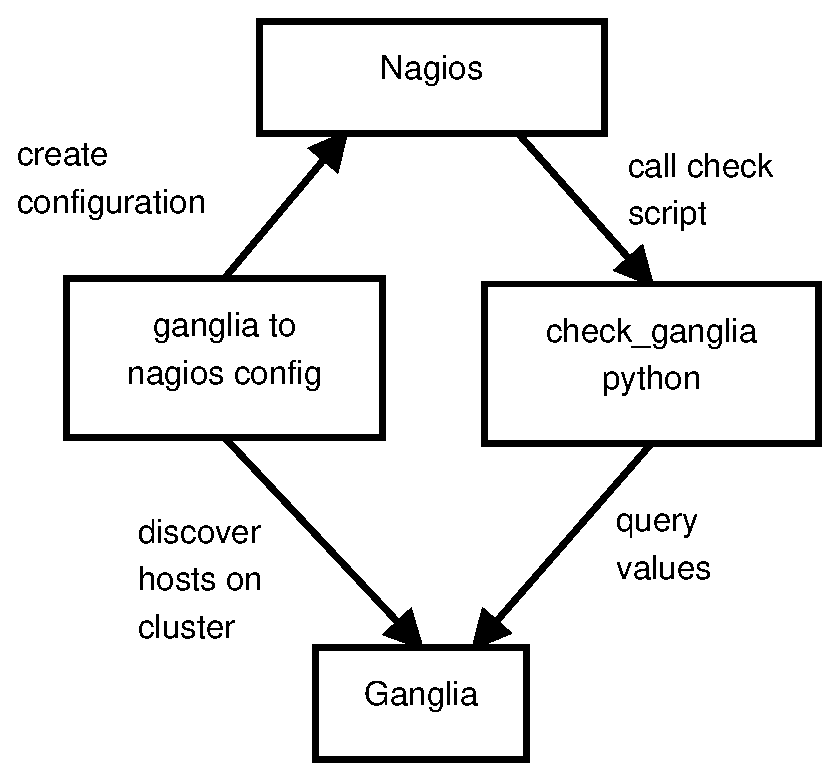
\includegraphics[width=2in]{images/nagios_check_ganglia.eps}
\caption{Nagios configuration and check ganglia values}
\label{figure:nagios_ganglia}
\end{figure}
\newpage

\subsection{pnp4nagios}

Bulk Mode with NPCD
NPCD:
spool directory to process bulk data
create graphs using RRDTOOL

\begin{figure}[htb]
\centering
 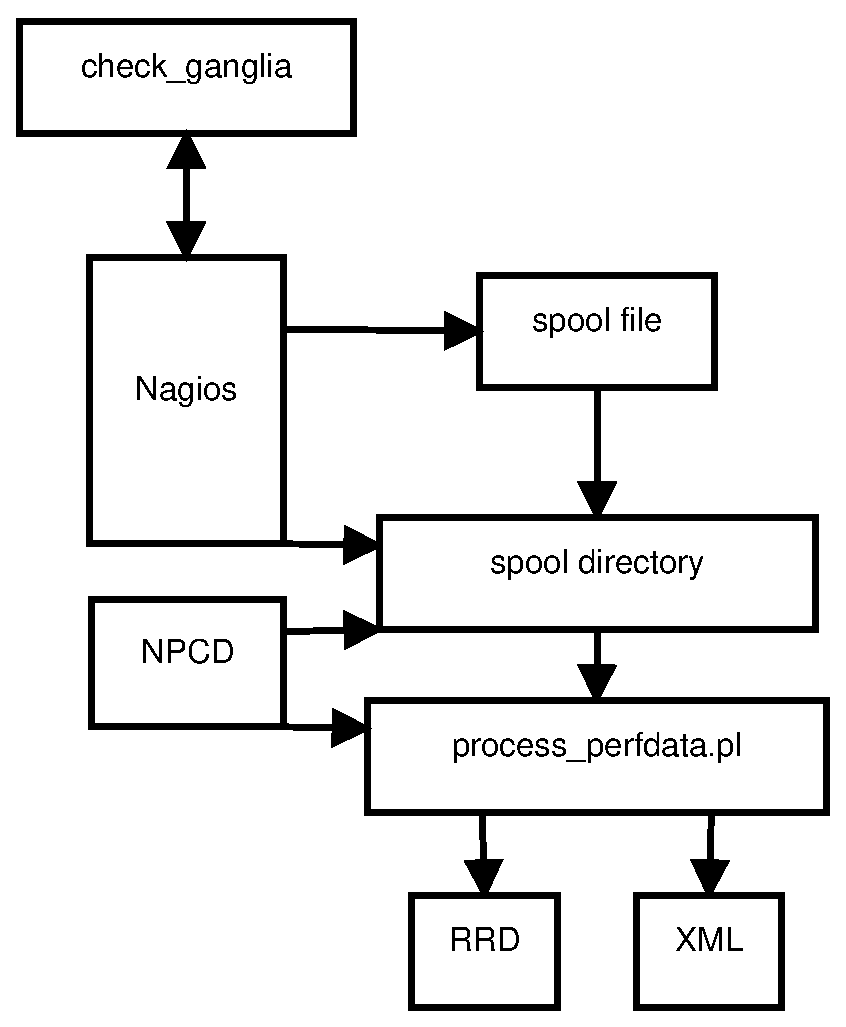
\includegraphics[width=3in]{images/npcd_pnp4nagios.eps}
\caption{PNP 4 Nagios data flow}
\label{figure:pnp4nagios}
\end{figure}
\newpage

\section{Range of cases examined - Metrics}
% here there will be an enumeration of metrics, gmond, etc

Grid performance can be measured using benchmark tools in different levels of the grid architecture, using the micro-benchmarks at the Worker Node level, the Site (CE) level and the Grid VO level. Various benchmarks exist in these levels, using different libraries and algorithms, such as This project focuses on mathematically compute of the performance of a grid based on the metrics that are taken at the Worker Node level.

Different metrics and benchmarks exist, such as the measurement of the performance of CPUs in {\bf MIPS using EPWhetstone} and the evaluation of the performance of a CPU in {\bf FLOP/s and MB/s using BlasBench}. GridBench \cite{gridbench} provides a framework to collect those metrics using its own description language, {\bf GBDL}.

GcpSensor \cite{gcpsensor} introduce a new performance metric called WMFLOPS. It uses PAPI \cite{papi} (Performance API) to access the hardware performance counters. For data distribution it uses MDS information system which provides dynamic metrics for CPU load average, one for 1, for 5 and for 15 minutes load.
\newpage

% TODO ganglia to MDS
\section{Publish to Information System}
\cite{goelagent}

\subsection{LDAP based - MDS/BDII}
To integrate Ganglia with MDS in early versions of Globus, there schema of OpenLDAP should be extended using the Glue-CE definitions from the DataTAG web site (MDS version 2.4). A Ganglia Information Provider was the native ganglia client on python, given by the ganglia development team itshelf.
\begin{enumerate}
  \item Python ganglia client script: \url{http://globus.org/toolkit/docs/2.4/mds/gangliaprovider.html}
  \item Perl gaglia-IP tool: \url{http://www.star.bnl.gov/public/comp/Grid/Monitoring/SimpleGangliaIP.html} and \url{http://www.star.bnl.gov/public/comp/Grid/Monitoring/ganglia\_ip}

\end{enumerate}

\newpage

\begin{table}[ht]
\begin{tabular}{ | l | l | r |}
\hline
{\bf Common Name} & {\bf Attribute} & {\bf Objectclass} \\ \hline
Hostname & GlueHostName & GlueHost \\ \hline
Unique ID assigned to the host & GlueHostUniqueID & GlueHost  \\ \hline
Processor Load, 1 Min Average  & GlueHostProcessorLoadLast1Min & GlueHostProcessorLoad \\ \hline
Processor Load, 5 Min Average  & GlueHostProcessorLoadLast5Min & GlueHostProcessorLoad \\ \hline
Processor Load, 15 Min Average  & GlueHostProcessorLoadLast15Min & GlueHostProcessorLoad \\ \hline
SMP Load, 1 Min Average  & GlueHostSMPLoadLast1Min & GlueHostSMPLoad \\ \hline
SMP Load, 5 Min Average  & GlueHostSMPLoadLast5Min & GlueHostSMPLoad \\ \hline
SMP Load, 15 Min Average  & GlueHostSMPLoadLast15Min & GlueHostSMPLoad \\ \hline
Number of CPUs  & GlueHostArchitectureSMPSize & GlueHostArchitecture \\ \hline
Processor Clock Speed (MHz)  & GlueHostProcessorClockSpeed & GlueHostProcessor \\ \hline
Network Interface name  & GlueHostNetworkAdapterName & GlueHostNetworkAdapter \\ \hline
Network Adapter IP address  & GlueHostNetworkAdapterIPAddress & GlueHostNetworkAdapter \\ \hline
The amount of RAM  & GlueHostMainMemoryRAMSize & GlueHostMainMemory \\ \hline
Free RAM (in KBytes)  & GlueHostMainMemoryRAMAvailable & GlueHostMainMemory \\ \hline
\end{tabular}
\caption{GLUE schema for Host Processor Information Provider}
\label{tab:tasks}
\end{table}

Perl:
\begin{lstlisting}
$[root@mon ~]# ./ganglia_ip -h mon -p 8649 -o mds
\end{lstlisting}

Python:
\begin{lstlisting}
$[root@mon ~]# /opt/ganglia/bin/ganglia --format=MDS
\end{lstlisting}

\begin{lstlisting}

[root@osweb ~]# cat /opt/glite/etc/gip/provider/glite-info-provider-service-ganglia-wrapper
#!/bin/bash
/opt/bin/ganglia_ip -h 195.251.70.54 -p 8649 -o mds
\end{lstlisting}

\newpage

\subsection{Web Service based - WSRF}
\subsubsection{container}
using WSRF (GT4, information services, information providers)
Ganglia Resource Provider
MDS Index Service
GLUE CE 

OASIS standard

container
\begin{figure}[htb]
\centering
 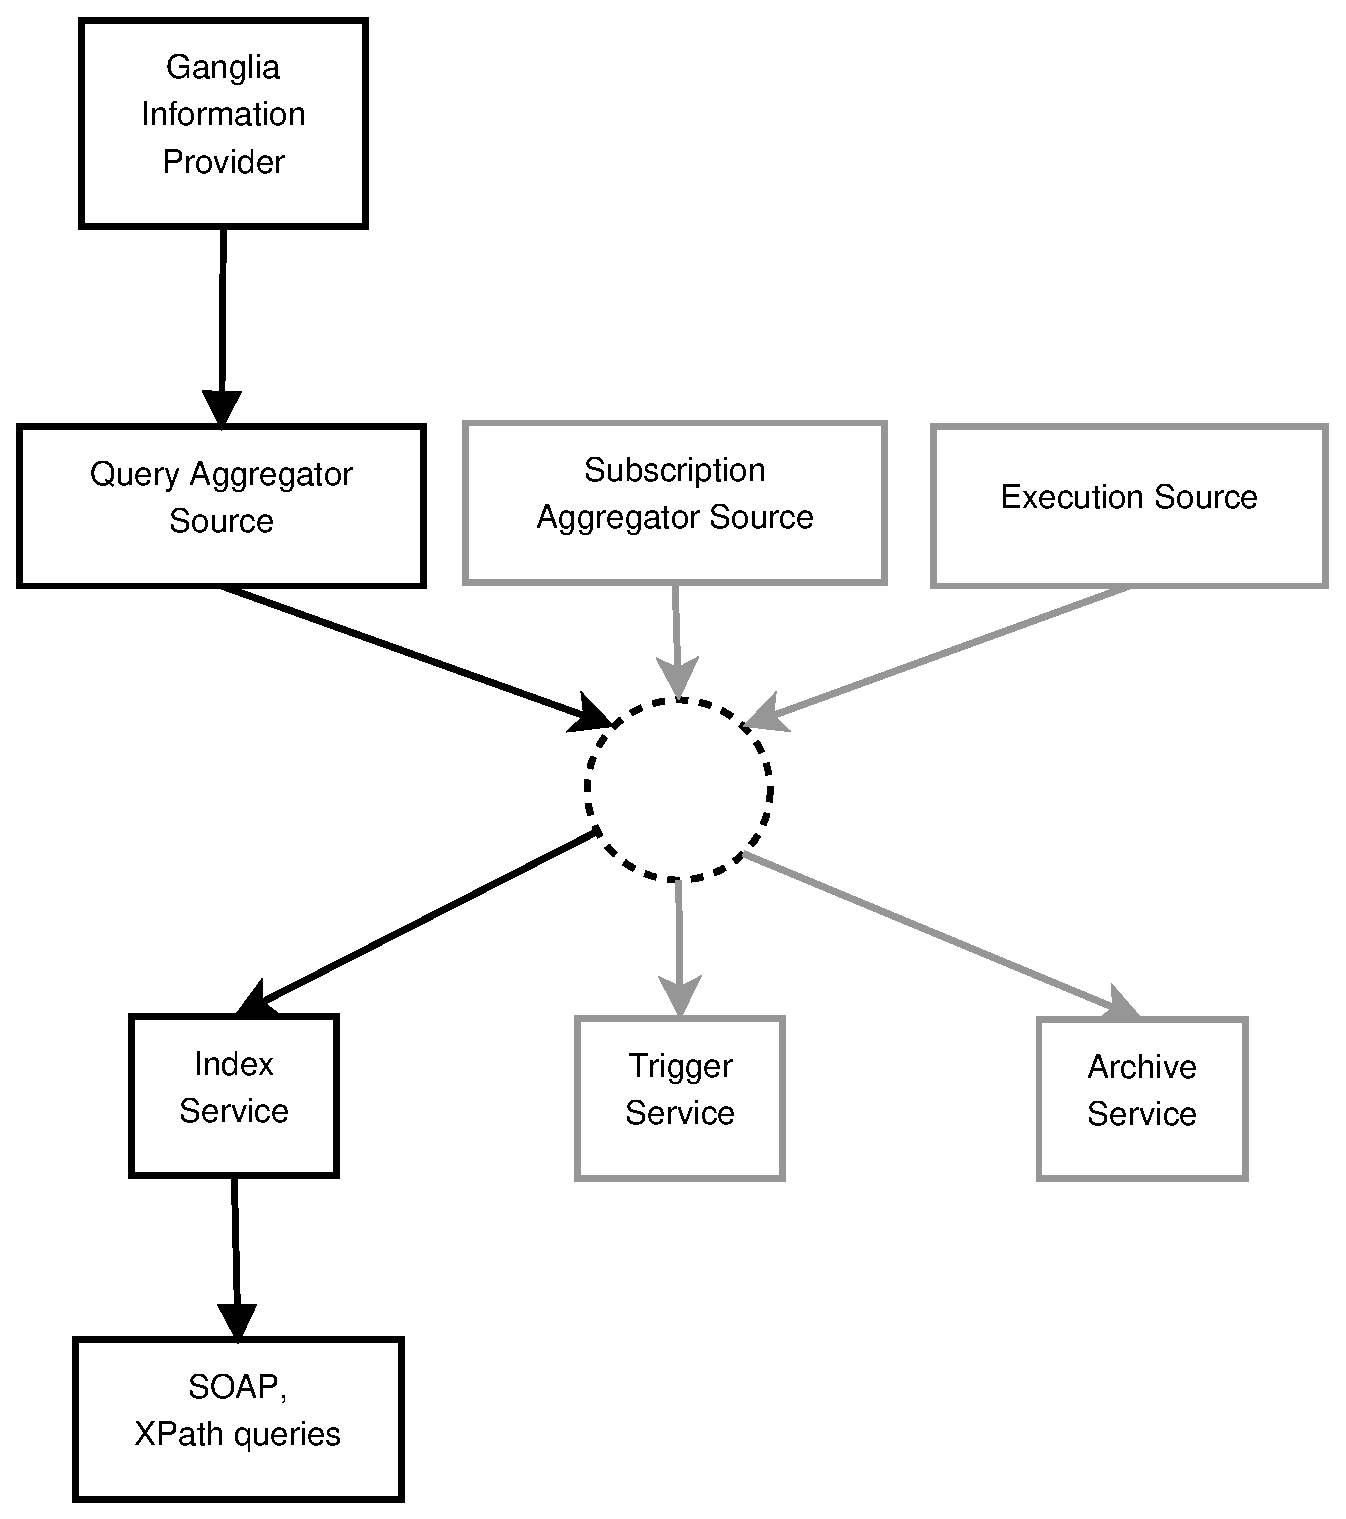
\includegraphics[width=5in]{images/wsrf.eps}
\caption{Web Service Resource Framework}
\label{figure:wsrf}
\end{figure}
\newpage
\subsection{information provider}
wssd

kai

rp xml

\newpage
\subsubsection{XPath}

XPath is used to parse an XML document and get a part of it using an address scheme. For XPath, the XML document is a tree consisting of nodes, and its purpose as a language is to get the nodes that are addressed using the XPath query from that document.

Its syntax is compact, non-XML and much like the filesystem addressing, so it facilitates the use of XPath within URIs.

Example queries used in this project are:

The following is used in the PHP code that queries the WebMDS for all nodes of the XML of the WSRF containing nodes with name $Host$:
\begin{verbatim}
//*[local-name()='Host']
\end{verbatim}

Another example is a more complex query that asks the WSRF for all nodes with name $Host$ that contains a sub-node named $ProcessorLoad$ and its $Last15Min$ attribute has value larger than 20:
\begin{verbatim}
//glue:Host[glue:ProcessorLoad[@glue:Last15Min>20]]
\end{verbatim}

Finally the following example may return only the $ProcessorLoad$ node of the $Host$ that has the attribute Name set to $xenia.oslab.teipir.gr$:
\begin{verbatim}
//glue:Host[@glue:Name='xenia.oslab.teipir.gr']/glue:ProcessorLoad
\end{verbatim}

\newpage

\subsubsection{XSLT}
my note: WSRF is GLUE 2.0 schema CE compatible
\begin{verbatim}
/opt/globus/etc/globus_wsrf_mds_usefulrp/ganglia_to_glue.xslt

<glue:ProcessorLoad>

<xsl:attribute name="glue:Last1Min">
  <xsl:call-template name="emitProperNumeric">
    <xsl:with-param name="numeric" 
    select="floor(100 * METRIC[@NAME='load_one']/@VAL)"/>
  </xsl:call-template>
</xsl:attribute>

<xsl:attribute name="glue:Last5Min">
  <xsl:call-template name="emitProperNumeric">
    <xsl:with-param name="numeric" 
    select="floor(100 * METRIC[@NAME='load_five']/@VAL)"/>
  </xsl:call-template>
</xsl:attribute>

<xsl:attribute name="glue:Last15Min">
  <xsl:call-template name="emitProperNumeric">
    <xsl:with-param name="numeric" 
    select="floor(100 * METRIC[@NAME='load_fifteen']/@VAL)"/>
  </xsl:call-template>
</xsl:attribute>

</glue:ProcessorLoad>
\end{verbatim}
\newpage

\subsubsection{WebMDS}
webmds

\chapter{Results}
\section{Tables and Plots}
\subsection{Visualization}
Drill down and levels of visualization
\begin{enumerate}
  \item local resource
  \item site
  \item regional
  \item grid
\end{enumerate}
\section{Methods of Presentation}
\subsection{Drill down approach}
ganglia graphs
\section{Description of Information}

\chapter{Analysis}
\section{Methods Adopted}

In complex distributed systems such as grids, performance bottlenecks may be located using monitoring data. From the processor usage on a single node of a computing element to the total usage of processed jobs in a large cluster, performance data help to focus on the problem that impacts the overall performance.

In order to succeed in grid monitoring, some requirements should be considered. A very large amount of data should be delivered real-time, from many heterogeneous sources on different networks or even countries. These data must be accurate and consistent. There should be synchronized timestamps on the generation of each metric, to the measurement value that should be comparable between different architectures. The time synchronization of the hosts of each cluster may be done using network time protocol, so all metrics are taken on the time that they actually report. Metrics should have error bounds to preserve accuracy, and the consistency issue is solved using coordination of that activity, so the impact of a metric to other sensors is controlled.

The flow of the monitoring process initialization is described from the GMA standard. The application-consumer queries the directory service in order to declare its interest to get metrics for a specific host/cluster. The sensors of the elements that is equivalent to the specific query generates the metrics that will be given to the consumer from the producer, which in turn queries the directory service to find the consumer. The producer is the one that initializes the connection to the consumer in order to deliver the measurements, even if the consumer had asked the directory service for this. \cite{balatonuse}


\subsection{Performance Metrics}

CALC\_LOAD - load average

extra
\subsubsection{Transport and sample}
Gmond code uses the ganglia libmetrics library which in case of Linux operating system parses the $/proc/loadavg$ pseudo-file to get linux kernel calculated system load average.

\begin{lstlisting}[language=C,caption=libmetrics code to get load average]
timely_file proc_loadavg = { {0,0} , 5., "/proc/loadavg" };
/* ... */
g_val_t
load_one_func ( void )
{
   g_val_t val;
   val.f = strtod( update_file(&proc_loadavg), (char **)NULL);
   return val;
}
\end{lstlisting}
code from gmond client

\subsection{Information Systems}

\subsubsection{BDII}

values left as decimal numbers because its easy for ldap to handle string values of numbers

\subsubsection{WSRF}

The XML that Ganglia Resource Provider took from Gmond process through TCP, using XSLT technology is transformed on WSRF to another XML document, that is following the Glue-CE schema. globus\_wsrf\_mds\_usefulrp directory of globus configuration root, there is the file ganglia\_to\_glue.xslt where we can focus on the transformation rules. A snippet of interest for the case of ProcessorLoad class is seen in Listing \ref{xslt}.

there is some XPath and a multiplication with 100 to get an integer that should be mentioned:

\begin{lstlisting}[language=XML,caption=WSRF XSLT for Ganglia Information Provider,label=xslt]
<glue:ProcessorLoad>

<xsl:attribute name="glue:Last1Min">
  <xsl:call-template name="emitProperNumeric">
    <xsl:with-param name="numeric" 
    select="floor(100 * METRIC[@NAME='load_one']/@VAL)"/>
  </xsl:call-template>
</xsl:attribute>

<xsl:attribute name="glue:Last5Min">
  <xsl:call-template name="emitProperNumeric">
    <xsl:with-param name="numeric" 
    select="floor(100 * METRIC[@NAME='load_five']/@VAL)"/>
  </xsl:call-template>
</xsl:attribute>

<xsl:attribute name="glue:Last15Min">
  <xsl:call-template name="emitProperNumeric">
    <xsl:with-param name="numeric" 
    select="floor(100 * METRIC[@NAME='load_fifteen']/@VAL)"/>
  </xsl:call-template>
</xsl:attribute>

</glue:ProcessorLoad>
\end{lstlisting}

\subsection{Nagios}

\begin{lstlisting}
define command{
 command_name  check-ganglia
 command_line  check_ganglia.py -h $HOSTNAME$ -m $ARG1$ \
               -w $ARG2$ -c $ARG3$ -s 195.251.70.54 -p 8649
 }

define service{
   use                  wn
   hostgroup_name       worker-nodes
   service_description  load_one
   check_command        check-ganglia!load_one!4!5
   action_url           https://osweb.teipir.gr/nagios/html/pnp4nagios/index.php?host=$HOSTNAME$&srv=$SERVICEDESC$
   }
\end{lstlisting}

\section{Interpretation of Results}


Discussion about performance results based on
load average.

some UNIX internals, processes, scheduler
not a percentage counter of CPU usage


Difference between these metrics and the availability of 
a grid based on the queue of jobs have been submitted.

Availability monitoring

-MyEGI, monitor visualization environment
-django data models
-MRS database, ATP based schema


\section{Specific Interpretations}

\subsection{Scaling}
\subsubsection{LDAP}

there is a paper about how information systems perform in large scale

LDAP as the core technology of MDS2 has been investigated \cite{zhang2004performance} and proved that scales and performs good when the data are kept in cache. The performance of the information system when it is accessed by a large number of cocurrent users have degrades dramatically when data caching is not used.

\subsubsection{WSRF}
deserialization of MDS query in gmond to WSRF

performance analysis of WSRF here \cite{schopf2006monitoring}

and MDS4 vs MDS2

\section{Enveloping Interpretations}

\chapter{Conclusions}
% chapter Conclusions

Grid monitoring is an important factor when working with Grid Systems. Reports extracted from monitoring systems, support decisions for capacity management, and prove that a system meets requirements needed for Service Level Agreements.

Metrics for Computing Element performance monitoring usually are:

\begin{enumerate}
 \item {\bf Total Jobs} in running or waiting to run state.
 \item Individual per working node {\bf Processor Load}.
 \item {\bf Benchmarking} metrics such as FLOP/s.
\end{enumerate}

This project focused in the calculation, aggregation and transfer to present the metrics for Processor Load of working nodes of a Computing Element. Running and waiting jobs monitoring is extremely analyzed under availability monitoring research.

Calculation using the number of processes waiting in the queue of kernel scheduler were used. It is explained why this metric is more accurate than the classic percentage CPU usage.

Aggregation and transfer of metrics where examined in many different levels, from the multicasted XDR of Gmond to the resource providers of the information service that were used.

Information Service is core technology that used in Grid Computing. It has evolved in parallel with Middleware. Current version of the Monitoring and Discovery Service standard has reached the MDS4, introducing the use of Web Services. MDS2 was based in LDAP, which is still used by some systems to discover services.

Nagios bulk aggregation features using NPCD and MSG-Nagios-Bridge also provide a method to aggregate Ganglia metrics without the use of the MDS.

Presentation were simply examined using:

\begin{enumerate}
 \item {\bf DOM technology} to parse XML taken from WSRF through WebMDS interface using XPath
 \item simple {\bf LDAP} communication to take the metrics from the BDII Information Service
\end{enumerate}

\section{Conclusions}

Every aspect of grid monitoring keeps {\bf scalability in mind}. Distribution of metrics in all worker nodes using Gmond is the key to keep redundant that information.

BDII Information Service is great for use in site level environment, as LDAP performs faster than WSRF in less than a hundred users.

Site monitoring needs Nagios and Ganglia for a few hundreds of nodes. Nagios web interface is enough for site-level host and service view. Ganglia web interface supports good aggregation of many clusters, to the Region-level.

WSRF caching feature, Indexer and Aggregator Framework scales better and may be used for regional and top level monitoring.

Heterogeneous environments should {\bf rely on standards} in order to inter-operate and stay reliable. Even the Information Services mentioned above stick to the Glue schema.

A tool may seem to be great for its purpose, but after focusing on a need is may be discontinued, such as SAM. This example is taken from the availability monitoring, as its frontend was replaced by MyEGI and Nagios keeping its back-end in MRS.

\section{Further Work}

\subsection{Aggregation}

Additional investigation is required to be carried out for the aggregation of collected information. WSRF offer the Aggregator Framework, which downstream information from many EPRs and deliver it through the Index service. Scaling such information in the Regional monitoring level may introduce issues that only in that scale will be visible.

\subsection{Benchmarking}

Performance metrics which are produced using benchmarking software is a good standard way of measuring and advertising the performance of Computing Elements. Such metrics are not efficient for regularly runs and frequent changes because they are cost effective performance wise. It is good although to present the performance ability of a CE. Rare periodic execution and push in the information service, will offer a good metric to select one CE of another.

\subsection{Storage element performance monitoring}

Storage Element performance monitoring is an interesting area for research. Vendors that produce enterprise level storage systems also offer tools to monitor the performance of the storage system. The most used metric is I/O Operations per second and throughput in GByte per second, in every aspect of a storage system.

Storage systems are also provided by different vendors and may also be deployed as custom solution. Fiber Channel solutions versus Clustered File System cases are examined \cite{brzezniak2008analysis} as a chapter of distributed systems, storage oriented.

Hadoop is the most commonly used distributed data storage. In CMS, an experiment that is known for its huge needs in data storage, Hadoop has been adopted \cite{hadoop} as the distributed file system. Grid computing community has adopted the use of Total and Used GB per Storage Element (as in Computing Element), but there is still enough work on the performance monitoring.



\backmatter

\bibliographystyle{ieeetr}
\nocite{*}
\bibliography{extra/books}

%\label{appb}
%\lhead{Appendix B. \emph{Interim Report}}
%\section{Introduction}

In EGI era of grid computing in Europe, MyEGEE and Nagios are taking the place of SAM in performance monitoring of the grid, in NGI oriented infrastructures. SAM Framework had a significant role in reporting the service availability. That monitoring model was needed to be replaced by a new Multi Level Monitoring architecture. The need of establishing a central point in regional level, where metrics gathered from each information system of the grid, lead to the adoption of MyOSG. MyEGEE is the tool that extends MyOSG to European NGI's and provides an interface to customize the display of aggregated metrics of the performance of NGI sites. Nagios is the main technological choice to provide that regional monitoring system.

\section{Aims and Objectives}

Different role users are going to use a portal to get information about the performance status of the grid, to export the appropriate report for their job. This project aims to develop these particular pieces of code to support the aggregation of the metrics from Nagios, to allow the web based customization of the visualization of the reports. These metrics are needed to report the availability and reliability of NGIs and particular sites of the grid.

The procedures that are going to be used in order to achieve the above aims should include at the beginning some opening and exploration of the environment where the interface is going to be placed. The usage of grid computing in the world should be well known, so a visibility of the importance and the possible uses of the software will be recognized. The appropriate access to the infrastructure should be gained, on different platforms and levels. Brunel University site and GridPP/NGS VO at the beginning, as long as the UKI ROC operations may be a good point of collaboration with researchers to reach the bests possible requirements and data to analyze. The middleware used in both these VOs should be examined so with the knowledge of running projects and global usage of them may target to export better specifications. Existing operations on the grid should also be discovered. The European initiative milestones on the operations of the regional level should be considered as a route, and registration to news about the upcoming research projects that are going to use the grid should also be take place.

After that wide-opening to get the whole picture, a targeted and focused view should follow. Existing monitoring tools must be used to check the problems and search for requirements. The experience of SAM, Gridview, Gridmap, Gstat, GridICE, etc should be taken in order to merge their functionality as possible as it is. Information systems that already reside over the infrastructure, must also be learned. Standards and specifications should be examined, on how the message bus works and delivers the data in an hierarchical manner. A contact with the CERN team working on MyEGEE and Indiana University's MyOSG team should be established, to collaborate on the core of MyOSG source. Changes submission to subversion system as long as ticket closure of the development project tool will help to get to know the core of MyEGEE and Nagios. It is possible to create and upstream a Nagios customized web interface, to create different views of Nagios resources scheme to grid topology oriented architecture. Nagios, NRPE and Ganglia installations should be deployed across the CE\&SE nodes of Brunel's sites to have a working production environment to work on. Attention should be taken on the potential performance impact of these sensors deployment. UKI MyEGEE validation/testing portal will be used as a pre-production environment to check changes. PNP should be fixed in GridPP Nagios to be evaluated. Statistical access log analysis of existing tools may have results on trends of users/admins preferred views.

Various tools are going to be used to track changes and collaborate. Monitoring articles in GridPP wiki \& CERN twiki should be made. Snippets upstream \& status changes must be a regular operation in SVN/JIRA/Trac in CERN interfaces. Ongoing task through the dissertation project is the reading of papers and methodical updates of Mendeley citation management tool to have the bibliography organized. Possible changes suggestions to MSc on DCS course notes about grid monitoring may by made, as long as the EGI roadmap updates. Finally with the appropriate supervision and follow-up of meetings and presentations, a paper publishing might take place.

\section{Literature Review}

Grid computing \cite{li2005grid} is the most recent decade's technology innovation in high performance computing. A large number of scientists working on the operations of this huge co-operative project of EU. Monitoring \& information architecture \cite{fisher2002datagrid} has been standardized in the initial state of that project, to succeed in today scale of 150.000 cores. Use of grid computing nowadays takes place in academic and research environments, but applications in industry-based needs such as promising Power Grid control \cite{Taylor2006} are emerging.

Standards are being published about the operational models that the grid computing initiative will use. Last decade the EGEE I, II \& III was adopted by european universities to fund and establish a collaborative community of researchers under a central point, the CERN oriented research project in Particle Physics. After EGEE, the European Grid Initiative were formed to lead to the explode of that community into regional initiatives. Performance and availability monitoring tools and views also follow that format, phasing out commonly used SAM \cite{egee3dsa122} and having the adoption of Nagios as the monitoring of regional performance tool.

Resource Brokers \cite{Kertesz06ataxonomy} where developed to manage the workload on Computer elements and Resource elements. Globus which is non-service based RB was replaced by gLite RB which is service based. A Workload Management System (WMS) exists in gLite to do the distribution and management of the Computing and Storage oriented tasks.

A Grid Monitoring Architecture \cite{tierney2002grid} was proposed in early 2000's. Information systems were developed to create repositories of information needed to be stored for monitoring and statistical reporting reasons. Such an organized system later was specified by the Aggregated Topology Provider (ATP) definition. The largest world grids adopt that model, forming OIM in OSG (USA) and GOCDB as that information base in EGEE (Europe). Message Bus was also defined as a mean to transfer the underlying data, and well known tools came up such as Gstat, GOCDB and BDII with Glue specification. Grid performance monitoring and keeping of such an information system has also impact in the performance of the system it shelf \cite{zhang2003performance}, so various methods were developed to give the solution to the scaling and performance problem, such as MDS2 (GIIS \& GRIS), GMA and R-GMA \cite{wilson2004information}, which offers relational environment \cite{fisher2001relational}, has experience on production systems \cite{byrom-production} and scales to reach huge needs such as CMS project \cite{Bonacorsi2004,Byrom}.

A taxonomy effort has been made \cite{gerndt2004performance} to present the differences of performance monitoring systems of the grid, and later a more general \cite{zanikolas2007importance} taxonomy paper was published to give a more general visibility of these tools. GridICE was generally used to aggregate the performance metrics of ROCs in high level reports \cite{andreozzi2005gridice}. Later GridICE was left as long as the SAM left, to meet the milestone of EGI to have a regional monitoring tool (Nagios) to report the reliability of the joined sites and report the values for SLA reasons. 

Latest EGI directive to form regional operation tools pushed the use of Nagios \cite{imamagic2007grid} as the main tools of availability \& performance (an so reliability) monitoring of the grid. Each NGI/ROC (regional level) has its own interface, and hierarchically there is a Super Nagios interface to report the top level view of general system availability. Nagios offers extensions such as NRPE to remotely invoke check commands in inaccessible/private installations. Another important add-on to Nagios is the NdoUtils, which offers an SQL store of history data to the monitoring interface. Nagios Configuration Generator was introduced to help the automatically generation of the configuration based on the information system of nodes and services. Finally, there has been proposed an integration of SAM views to a Nagios customized interface, to offer the last good known SAM interface to the old users. Nagios also integrates with GGUS, a ticketing system that european grid initiative uses.

Brunel University takes part in regional and european initiatives. 4 different Computer Elements exist, and 3 Storage Elements, consisting the UKI-LT2-Brunel site. LT2 stands for London Grid, a co-operation with other London Universities. GridPP and NGS are two collaboration groups that Brunel University is member of, and papers on the web interface \cite{Hobson2007} and real time visualization of the grid status were presented \cite{Huang2007} by GridPP.

\section[Experimental]{Experimental/investigative methods to be adopted}

To develop the interface of customized views of aggregated performance metrics, an initial evaluation of the underlying information systems must be made. Data repositories and technologies that specifies the message bus, such as LDAP/BDII, SQL/R-GMA, XML multicast/Ganglia and file logging/ndo2db-SQL of Nagios should be evaluated. 

The views that are needed, based on the appropriate roles (users, operators/admins, managers) must be specified before deciding which hierarchical model view will be chosen. There should be checked whether it is useful to layer the views to service/node/site/NGI/VO reports or to target to a specific.

The language that is going to be used to aggregate the underlying data should also be chosen at this point. MyEGEE is PHP based, Nagios core is based in open source CGI and plugins are bash/perl scripts. Nagios web interface plugins are usually in PHP/Python. The integration of Nagios and BDII using NCG should take care of exit status of Nagios commands, that should be interpreted numerical values of services/resources metrics. It is possible to create custom Nagios plugins-check scripts. 

The decision of how special graphs are going to be created should be also made. Using standard libraries such as rrdtool, or whether to aggregate the already generated by the new Gstat 2.0 graphs. There are also two ways of generation of the graphs. Generation of graphs may be followed by disk caching using files, or on demand generation using a PHP/python script throwing binary image headers to produce graphs. Mixed environment is another solution to exceed speed due to caching of common used graphs, and flexibility in rare reports. There should also be decided if Ganglia gmond/gmetad metrics are going to be aggregated in the MyEGEE. 

Finally, security using authentication should be checked in the whole tree of the portal, and performance tuning queries should be always be an ongoing task to reach the required scaling of use of the interface.

\begin{table}[ht]
\begin{tabular}{ | l | l | l | l | r |}
\hline
Task & Start date & End date & Duration in days \\ \hline
  Preliminary & 03/29/10 & 04/24/10 & 20 \\ \hline 
  -  Identify Concepts & 03/29/10 & 04/08/10 & 8 \\ \hline 
  -  Gain Access & 04/08/10 & 04/24/10 & 12 \\ \hline 
  Planning & 05/12/10 & 06/04/10 & 17 \\ \hline 
  -  Explore existing technologies & 05/12/10 & 05/28/10 & 12 \\ \hline 
  -  Write Interim Report & 05/28/10 & 06/04/10 & 5 \\ \hline 
  Experimental-Development & 06/04/10 & 08/14/10 & 51 \\ \hline 
  -  Evaluate performance monitoring tools & 06/04/10 & 06/25/10 & 15 \\ \hline 
  -  Information/topology databases & 06/17/10 & 06/29/10 & 8 \\ \hline 
  -  Develop Customized Interface & 06/29/10 & 08/14/10 & 34 \\ \hline 
  ---    Coding of information aggregation & 06/29/10 & 07/21/10 & 16 \\ \hline 
  ---    Development of the frontend & 07/21/10 & 08/10/10 & 14 \\ \hline 
  ---    Complete the interface (auth, scale, etc) & 08/10/10 & 08/14/10 & 4 \\
      \hline Report & 08/16/10 & 09/29/10 & 32 \\ \hline 
  -  Begin Writing & 08/17/10 & 09/01/10 & 11 \\ \hline 
  -  Submit Draft \& Make Changes & 09/01/10 & 09/14/10 & 9 \\ \hline 
  -  Prepare Final & 09/14/10 & 09/29/10 & 11 \\ \hline 
\end{tabular}
%\caption{Key activities necessary to complete the project}
\label{tab:tasks}
\end{table}


\section[Time plan]{Time-plan (Gantt Chart)}

\tikzstyle{line} = [draw]

\begin{tikzpicture}
%\draw[help lines] (0,0) grid +(10,1);
%lines
\draw (0,0) -- (0,-3.2);
%\path [line,dashed] (1,0) -- (1,-5.7);
\path [line,dashed] (2,0) -- (2,-3.2);
%\path [line,dashed] (3,0) -- (3,-5.7);
\path [line,dashed] (4,0) -- (4,-3.2);
%\path [line,dashed] (5,0) -- (5,-5.7);
\path [line,dashed] (6,0) -- (6,-3.2);
%\path [line,dashed] (7,0) -- (7,-5.7);
\path [line,dashed] (8,0) -- (8,-3.2);
%\path [line,dashed] (9,0) -- (9,-5.7);
\path [line,dashed] (10,0) -- (10,-3.2);
%\path [line,dashed] (11,0) -- (11,-5.7);
\path [line,dashed] (12,0) -- (12,-3.2);

\draw (-1.5,-0.5) node[above]{$ \textsc{Preliminary}$};%
\draw (-1.5,-1) node[above]{$ \textsc{Planning}$};%
\draw (-1.5,-1.5) node[above]{$ \textsc{Development}$};%
\draw (-1.5,-2) node[above]{$ \textsc{Evaluation}$};%
\draw (-1.5,-2.5) node[above]{$ \textsc{Interface}$};%
\draw (-1.5,-3) node[above]{$ \textsc{Report}$};%
%\draw (-1.5,-3.5) node[above]{$ \textsc{activity G}$};%
%\draw (-1.5,-4) node[above]{$ \textsc{activity H}$};%
%\draw (-1.5,-4.5) node[above]{$ \textsc{activity I}$};%
%\draw (-1.5,-5) node[above]{$ \textsc{activity J}$};%
%\draw (-1.5,-5.5) node[above]{$ \textsc{Report}$};%

\filldraw[fill=white] (0,-0.1) rectangle (3.42,-0.4);% a slack
\filldraw[fill=blue] (0,-0.1) rectangle (3.12,-0.4);% a
\filldraw[fill=white] (3.42,-0.6) rectangle (4.2,-0.9);% b slack
\filldraw[fill=blue] (3.42,-0.6) rectangle (4.2,-0.9);% b
\filldraw[fill=blue] (4.2,-1.1) rectangle (9,-1.4);% c
\filldraw[fill=white] (4.2,-1.6) rectangle (7.5,-1.9);% d slack
\filldraw[fill=blue] (4.2,-1.6) rectangle (6.5,-1.9);% d
\filldraw[fill=white] (7.5,-2.1) rectangle (9,-2.4);% e slack
\filldraw[fill=blue] (7.5,-2.1) rectangle (8.8,-2.4);% e
\filldraw[fill=white] (9,-2.6) rectangle (11.36,-2.9);% k slack
\filldraw[fill=blue] (9,-2.6) rectangle (11,-2.9);% k
%\filldraw[fill=white] (3.2,-2.6) rectangle (6.66,-2.9);% f slack
%\filldraw[fill=blue] (3.2,-2.6) rectangle (3.4,-2.9);% f
%\filldraw[fill=white] (7,-3.1) rectangle (9.6,-3.4);% g slack
%\filldraw[fill=blue] (7,-3.1) rectangle (8,-3.4);% g
%\filldraw[fill=white] (7,-3.6) rectangle (7.53,-3.9);% h slack
%\filldraw[fill=blue] (7,-3.6) rectangle (7.43,-3.9);% h 
%\filldraw[fill=blue] (6.66,-4.1) rectangle (7.53,-4.4);% i 
%\filldraw[fill=blue] (7.53,-4.6) rectangle (9.58,-4.9);% i 

\draw (0,-3.2) -- (12,-3.2);
\draw (0,-3.2) -- (12.1,-3.2);


\draw (-2,-4) node[above]{$ \textsc{Months}$};%
\draw (1,-4) node[above]{$ \textsc{Apr}$};%
%\draw (1,-6.5) node[above]{$ \textsc{21}$};%
\draw (3,-4) node[above]{$ \textsc{May}$};%
%\draw (3,-6.5) node[above]{$ \textsc{23}$};%
\draw (5,-4) node[above]{$ \textsc{Jun}$};%
%\draw (5,-6.5) node[above]{$ \textsc{25}$};%
\draw (7,-4) node[above]{$ \textsc{Jul}$};%
%\draw (7,-6.5) node[above]{$ \textsc{27}$};%
\draw (9,-4) node[above]{$ \textsc{Aug}$};%
%\draw (9,-6.5) node[above]{$ \textsc{29}$};%
\draw (11,-4) node[above]{$ \textsc{Sep}$};%
%\draw (11,-6.5) node[above]{$ \textsc{31}$};%
%\draw (12,-6.5) node[above]{$ \textsc{}$};%
\end{tikzpicture}



\pagebreak
\section[Deliverables]{Deliverables or specific outcomes}

\begin{itemize}
  \item Standards based monitoring environment for the UKI-LT2-Brunel site
  \item Site level Nagios web interface with PNP visualization graphs for the report of Nagios check commands, NRPE installations if needed for the different CEs/SEs for the UKI-LT2-Brunel
  \item Site level Ganglia monitoring. Gmond \& Gmetad installations in every node of every CE/SE of UKI-LT2-Brunel
  \item Region level customized MyEGEE, to offer basic customization of taken metrics. The aggregation should be made based on the previous SAM views. That MyEGEE will be installed in validation/testing UKI MyEGEE.
  \item Region level Nagios web interface, with PNP visualization graphs for the report of member-sites availability based on the taken metric at a higher level.
  \item A number of submissions to the MyOSG/MyEGEE project at Indiana University and CERN repositories.
\end{itemize}


\newpage
\thispagestyle{empty}
\begin{center}
\Large
School of Engineering \& Design\\
Electronic \& Computer Engineering\\
\vspace{0.5\baselineskip}
\begin{center}

\includegraphics[width=40mm]{images/brunel_logo.eps}\\
\end{center}
\Large
Industrial Mentor's Report on a MSc Dissertation\\
\end{center}
\Large
\vspace{0.5\baselineskip}
Student's name: Theofylaktos Papapanagiotou
\\
Dissertation Title: Grid Monitoring

\vspace{0.5\baselineskip}
\large
\noindent

I confirm / cannot confirm* that the MSc dissertation submitted by the above student truly reflects the respective contributions of the student and others, with whom the student has worked during the MSc project.

\vspace{0.5\baselineskip}
$*$ delete as appropriate

\vspace{1\baselineskip}
Comments:


\vspace{2.5\baselineskip}
\noindent
Signed:\\
Name: Dr.Paul Kyberd\\
Date:

\printindex

\end{document}
